%% ============================================================
%%  Cliente GPS IoT — External Pentest Report
%%  Autor: Clark Espinal
%%  Fecha: [REDACTED]
%% ============================================================
\documentclass[11pt,a4paper]{article}

\usepackage[utf8]{inputenc}
\usepackage[T1]{fontenc}
\usepackage[spanish]{babel}
\usepackage[margin=2.5cm, top=3cm, bottom=3cm]{geometry}
\usepackage{xcolor}
\usepackage{graphicx}
\usepackage{booktabs}
\usepackage{tabularx}
\usepackage{array}
\usepackage{enumitem}
\usepackage{fancyhdr}
\usepackage{titlesec}
\usepackage{hyperref}
\usepackage{listings}
\usepackage{tcolorbox}
\usepackage{multirow}
\usepackage{colortbl}
\usepackage{parskip}
\usepackage{tikz}
\usepackage{lmodern}
\usepackage[activate={true,nocompatibility},letterspace=150]{microtype}
\usepackage{caption}
\setlength{\headheight}{14.5pt}
\usetikzlibrary{shapes.geometric, arrows.meta, positioning, shadows}
\tcbuselibrary{skins, breakable}

%% Colores
\definecolor{critical}{HTML}{C0392B}
\definecolor{high}{HTML}{E67E22}
\definecolor{medium}{HTML}{D4AC0D}
\definecolor{low}{HTML}{27AE60}
\definecolor{darkbg}{HTML}{111827}
\definecolor{accentblue}{HTML}{4A90D9}
\definecolor{accentbluedark}{HTML}{1A3A5C}
\definecolor{lightgray}{HTML}{F5F6FA}
\definecolor{codebg}{HTML}{1E1E2E}
\definecolor{codetext}{HTML}{CDD6F4}
\definecolor{bordercolor}{HTML}{DDDDDD}
\definecolor{textmuted}{HTML}{6B7280}
\definecolor{textlight}{HTML}{9CA3AF}

\hypersetup{
    colorlinks=true,
    linkcolor=accentbluedark,
    urlcolor=accentblue,
    citecolor=accentbluedark,
    pdftitle={Puyu IoT GPS Platform — External Pentest Report},
    pdfauthor={Clark Espinal},
}

\lstset{
    backgroundcolor=\color{codebg},
    basicstyle=\ttfamily\footnotesize\color{codetext},
    breaklines=true,
    breakatwhitespace=false,
    columns=flexible,
    keepspaces=true,
    frame=single,
    framesep=5pt,
    rulecolor=\color{accentblue},
    xleftmargin=10pt,
    xrightmargin=10pt,
    aboveskip=8pt,
    belowskip=8pt,
    showstringspaces=false,
    inputencoding=utf8,
    extendedchars=false,
}

\pagestyle{fancy}
\fancyhf{}
\fancyhead[L]{\textcolor{accentblue}{\small\textsc{Puyu IoT GPS Platform --- External Pentest Report}}}
\fancyhead[R]{\textcolor{textmuted}{\small Clark Espinal $\cdot$ [REDACTED]}}
\fancyfoot[C]{\textcolor{textmuted}{\small\thepage}}
\renewcommand{\headrulewidth}{0.5pt}
\renewcommand{\footrulewidth}{0pt}
\renewcommand{\headrule}{\color{accentblue}\hrule width\headwidth height\headrulewidth}

\titleformat{\section}
  {\large\bfseries\color{accentbluedark}\scshape}
  {\thesection}{1em}{}[\vspace{2pt}\color{accentblue}\titlerule\vspace{4pt}]

\titleformat{\subsection}
  {\normalsize\bfseries\color{accentbluedark}}
  {\thesubsection}{1em}{}

\titleformat{\subsubsection}
  {\normalsize\bfseries\color{textmuted}}
  {\thesubsubsection}{1em}{}

%% ============================================================
\begin{document}
\raggedbottom
\pagenumbering{gobble}

%% ---- PORTADA ----
\begin{titlepage}
\pagecolor{darkbg}
\color{white}

\begin{tikzpicture}[remember picture, overlay]
  \fill[accentblue!60!darkbg] (current page.north west) rectangle +(\paperwidth, -0.35cm);
  \fill[accentblue!60!darkbg] (current page.south west) rectangle +(\paperwidth, 0.35cm);
\end{tikzpicture}

\vspace*{2cm}
\begin{center}

{\small\textls*[200]{\textcolor{accentblue}{\textsc{Offensive Security}}}}\\[1.2cm]

{\fontsize{28}{34}\selectfont\textsc{Puyu IoT GPS Platform}}\\[0.3cm]
{\fontsize{28}{34}\selectfont\textsc{\textcolor{accentblue}{External Pentest Report}}}\\[1.8cm]

{\small\textcolor{textlight}{\texttt{Black-box Assessment $\cdot$ Externo $\cdot$ 3 Hosts}}}\\[2.5cm]

{\color{accentblue!40}\rule{6cm}{0.4pt}}\\[2cm]

{\small\textcolor{textmuted}{Target}}\\[0.2cm]
{\normalsize\textcolor{white}{Puyu IoT GPS Platform}}\\[0.5cm]
{\small\textcolor{textmuted}{Hosts evaluados}}\\[0.2cm]
{\normalsize\textcolor{white}{\texttt{HOST-A $\cdot$ HOST-B $\cdot$ HOST-C}}}\\[0.5cm]
{\small\textcolor{textmuted}{Periodo}}\\[0.2cm]
{\normalsize\textcolor{white}{[REDACTED]}}\\[0.5cm]
{\small\textcolor{textmuted}{Tipo}}\\[0.2cm]
{\normalsize\textcolor{white}{Black-box $\cdot$ Externo $\cdot$ Sin credenciales previas}}\\[2cm]

{\small\textcolor{textmuted}{Autor}}\\[0.3cm]
{\normalsize\textcolor{white}{Clark Espinal}}\\[0.1cm]
{\small\textcolor{textlight}{Penetration Tester}}

\end{center}
\end{titlepage}

\nopagecolor
\pagenumbering{arabic}
\setcounter{page}{1}

%% ---- TOC ----
\thispagestyle{empty}
\begin{center}
{\large\bfseries\scshape\color{accentbluedark} Tabla de Contenidos}\\[0.3cm]
{\color{accentblue}\rule{4cm}{0.5pt}}
\end{center}
\vspace{0.3cm}
\tableofcontents
\newpage

%% ============================================================
\section{Resumen Ejecutivo}
%% ============================================================

Se realizo una prueba de penetracion externa sobre tres servidores de produccion
de la plataforma Cliente GPS IoT, operada bajo los dominios \texttt{[REDACTED]}
y \texttt{[REDACTED]}. La evaluacion fue de tipo caja negra, sin credenciales
previas, realizada desde internet publico durante el periodo \texttt{[REDACTED]}.

Se identificaron 16 hallazgos distribuidos en los tres hosts. El servidor
principal (\texttt{HOST-C}) concentra el mayor riesgo: una instancia
de Wiki.js accesible sin autenticacion expone la arquitectura completa del
sistema, incluyendo un script de acceso SSH como \texttt{root} al servidor
de produccion. Combinado con la ausencia de proteccion anti-bruteforce en SSH,
existe un vector directo hacia el compromiso total de la infraestructura.

\vspace{0.4cm}

\begin{tcolorbox}[colback=critical!8, colframe=critical, boxrule=1pt, arc=3pt,
  title={\textbf{Riesgo Critico Confirmado}},
  fonttitle=\bfseries\color{white}, coltitle=white, colbacktitle=critical]
La combinacion de Wiki.js publica con \texttt{tunnels.sh} expuesto y SSH root
sin rate limiting representa un vector de compromiso total del servidor GPS.
Un atacante externo puede lanzar un ataque de diccionario contra root usando
la IP y el usuario obtenidos directamente de la wiki sin necesidad de
reconocimiento adicional.
\end{tcolorbox}

\vspace{0.4cm}

\subsection*{Resumen de Hallazgos}

\begin{center}
\begin{tabular}{lc}
\toprule
\textbf{Severidad} & \textbf{Cantidad} \\
\midrule
Critico  & 3 \\
Alto     & 5 \\
Medio    & 5 \\
Bajo     & 2 \\
Info     & 1 \\
\midrule
\textbf{Total} & \textbf{16} \\
\bottomrule
\end{tabular}
\end{center}

\vspace{0.4cm}

\subsection*{Top 3 Hallazgos Criticos}

\begin{enumerate}[leftmargin=*, label=\textbf{\arabic*.}]
  \item \textbf{Wiki.js publica + tunnels.sh expuesto (F-C-01 / F-C-02)} ---
    La wiki de documentacion tecnica es accesible sin autenticacion desde
    internet. Contiene el script \texttt{tunnels.sh} con la IP publica del
    servidor y el usuario \texttt{root}, exponiendo el vector de acceso SSH
    al servidor de produccion completo.

  \item \textbf{Grafana con credenciales por defecto admin:admin (F-B-01)} ---
    El panel de Grafana acepta \texttt{admin:admin}. Otorga acceso administrativo
    completo incluyendo datasources de PostgreSQL con cadenas de conexion
    a bases de datos internas.

  \item \textbf{SSH root sin proteccion anti-bruteforce (F-C-08)} ---
    El servidor principal acepta autenticacion por contrasena para \texttt{root}
    sin bloqueo de IP ni rate limiting. Durante la prueba se realizaron mas
    de 2000 intentos con hydra sin respuesta defensiva del servidor.
\end{enumerate}

\newpage

%% ============================================================
\section{Alcance y Metodologia}
%% ============================================================

\subsection{Alcance}

\begin{center}
\begin{tabularx}{\textwidth}{lX}
\toprule
\textbf{Elemento} & \textbf{Detalle} \\
\midrule
Tipo de prueba  & Black-box (sin credenciales previas) \\
Modalidad       & Externo --- desde internet publico \\
Autorizacion    & Prueba autorizada por el cliente \\
Periodo         & [REDACTED] \\
\midrule
Host A        & \texttt{HOST-A} --- Jenkins CI/CD \\
Host B        & \texttt{HOST-B} --- Grafana / Laravel / phpMyAdmin \\
Host C        & \texttt{HOST-C} --- GPS Platform / Wiki.js / Spring Boot \\
\bottomrule
\end{tabularx}
\end{center}

\subsection{Metodologia}

La evaluacion siguio las fases estandar de prueba de penetracion:

\begin{center}
\begin{tabular}{clll}
\toprule
\textbf{Fase} & \textbf{Nombre} & \textbf{Estado} & \textbf{Resultado} \\
\midrule
1 & Reconocimiento          & \textcolor{low}{\textbf{Completado}} & Puertos, servicios, fingerprinting \\
2 & Enumeracion             & \textcolor{low}{\textbf{Completado}} & Endpoints, GraphQL, directorios, SSL \\
3 & Analisis de vulns       & \textcolor{low}{\textbf{Completado}} & CVEs, credenciales por defecto, configs \\
4 & Explotacion (limitada)  & \textcolor{low}{\textbf{Completado}} & Acceso Grafana, Wiki, SSH bruteforce \\
5 & Documentacion           & \textcolor{low}{\textbf{Completado}} & 16 hallazgos clasificados con evidencia \\
\bottomrule
\end{tabular}
\end{center}

\subsection{Herramientas Utilizadas}

\begin{center}
\begin{tabular}{llp{7cm}}
\toprule
\textbf{Herramienta} & \textbf{Fase} & \textbf{Uso} \\
\midrule
\texttt{nmap}         & Recon       & Escaneo de puertos y deteccion de servicios \\
\texttt{whatweb}      & Recon       & Fingerprinting de tecnologias web \\
\texttt{curl}         & Enum        & Inspeccion de cabeceras y endpoints HTTP \\
\texttt{feroxbuster}  & Enum        & Enumeracion de directorios \\
\texttt{nuclei}       & Analisis    & Deteccion automatizada de vulnerabilidades \\
\texttt{hydra}        & Explotacion & Prueba de rate limiting en SSH \\
\texttt{mysql-client} & Explotacion & Verificacion de acceso a MySQL expuesto \\
\bottomrule
\end{tabular}
\end{center}

\newpage

%% ============================================================
\section{Hallazgos --- Host A (HOST-A) --- Jenkins}
%% ============================================================

Servicio principal: Jenkins 2.555.2.
Puertos identificados: 8080 (Jenkins), 443 (HTTPS).

\vspace{0.3cm}

%% ---- F-A-01 ----
\subsection{F-A-01 --- Version de Jenkins expuesta publicamente}

\begin{tcolorbox}[colback=lightgray, colframe=bordercolor, boxrule=0.5pt, arc=3pt,
  title={\textbf{F-A-01} \hfill \textbf{INFO $\cdot$ CWE-200}},
  fonttitle=\bfseries, breakable]

\textbf{Host:} \texttt{HOST-A:8080}\\[4pt]

\textbf{Descripcion:}
La version exacta de Jenkins (2.555.2) es visible en las cabeceras HTTP
y en la interfaz web sin autenticacion. Esto permite identificar CVEs
especificos aplicables a la version instalada sin necesidad de acceso previo.

\begin{lstlisting}
whatweb http://HOST-A:8080
# Jenkins[2.555.2] X-Jenkins[2.555.2] X-Jenkins-Session[...]
\end{lstlisting}

\begin{center}
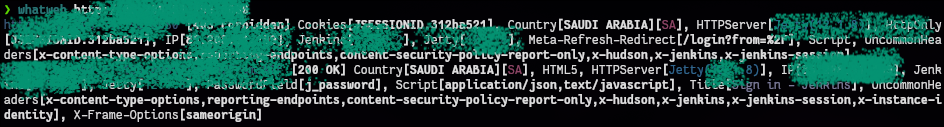
\includegraphics[width=0.82\textwidth]{../evidence/screenshots/199-whatweb-output.png}
\captionof*{figure}{\small\textcolor{textmuted}{whatweb --- version Jenkins 2.555.2 expuesta en cabeceras}}
\end{center}

\textbf{Remediacion:}
\begin{itemize}[noitemsep]
  \item Ocultar la version en cabeceras HTTP desde la configuracion de Jenkins.
  \item Mantener Jenkins actualizado a la ultima version estable disponible.
\end{itemize}
\end{tcolorbox}

\vspace{0.4cm}

%% ---- F-A-02 ----
\subsection{F-A-02 --- Jenkins CLI accesible sin autenticacion}

\begin{tcolorbox}[colback=low!6, colframe=low, boxrule=1pt, arc=3pt,
  title={\textbf{F-A-02} \hfill \textbf{BAJO $\cdot$ CWE-306}},
  fonttitle=\bfseries\color{white}, coltitle=white, colbacktitle=low, breakable]

\textbf{Host:} \texttt{HOST-A:8080}\\[4pt]

\textbf{Descripcion:}
El endpoint \texttt{/jnlpJars/jenkins-cli.jar} es descargable sin autenticacion.
El CLI permite ejecutar comandos limitados de enumeracion remota sin credenciales
validas, ampliando la superficie de ataque disponible para un actor externo.

\begin{lstlisting}
curl -sk http://HOST-A/jnlpJars/jenkins-cli.jar -o jenkins-cli.jar
java -jar jenkins-cli.jar -s https://HOST-A -noCertificateCheck -https
\end{lstlisting}

\begin{center}
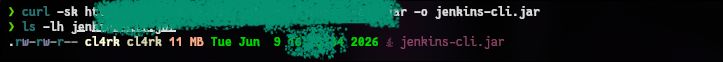
\includegraphics[width=0.82\textwidth]{../evidence/screenshots/199-jenkins-cli-jar-download.png}
\captionof*{figure}{\small\textcolor{textmuted}{Descarga de jenkins-cli.jar sin autenticacion}}
\end{center}

\begin{center}
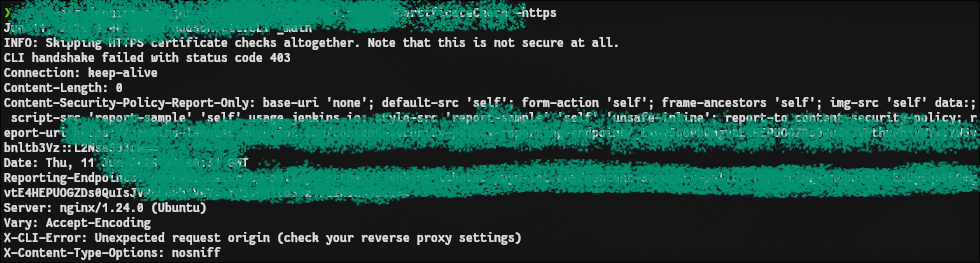
\includegraphics[width=0.82\textwidth]{../evidence/screenshots/199-curl-cli-verbose.png}
\captionof*{figure}{\small\textcolor{textmuted}{Ejecucion de comandos CLI sin credenciales}}
\end{center}

\textbf{Remediacion:}
\begin{itemize}[noitemsep]
  \item Requerir autenticacion para acceder al endpoint del CLI.
  \item Deshabilitar el acceso remoto al CLI si no es necesario operacionalmente.
\end{itemize}
\end{tcolorbox}

\vspace{0.4cm}

%% ---- F-A-03 ----
\subsection{F-A-03 --- CVE-2024-23897 (LFI en Jenkins CLI) --- Mitigado}

\begin{tcolorbox}[colback=low!6, colframe=low, boxrule=1pt, arc=3pt,
  title={\textbf{F-A-03} \hfill \textbf{BAJO (mitigado) $\cdot$ CVE-2024-23897 $\cdot$ CWE-22}},
  fonttitle=\bfseries\color{white}, coltitle=white, colbacktitle=low, breakable]

\textbf{Host:} \texttt{HOST-A:8080}\\[4pt]

\textbf{Descripcion:}
Se intento explotar CVE-2024-23897, una vulnerabilidad de lectura arbitraria
de archivos en Jenkins CLI que afecta versiones anteriores a 2.442. El servidor
bloqueo el intento, indicando que el control esta implementado. Sin embargo,
la exposicion del CLI sin autenticacion mantiene una superficie de riesgo
en caso de regresion o actualizacion mal gestionada.

\begin{center}
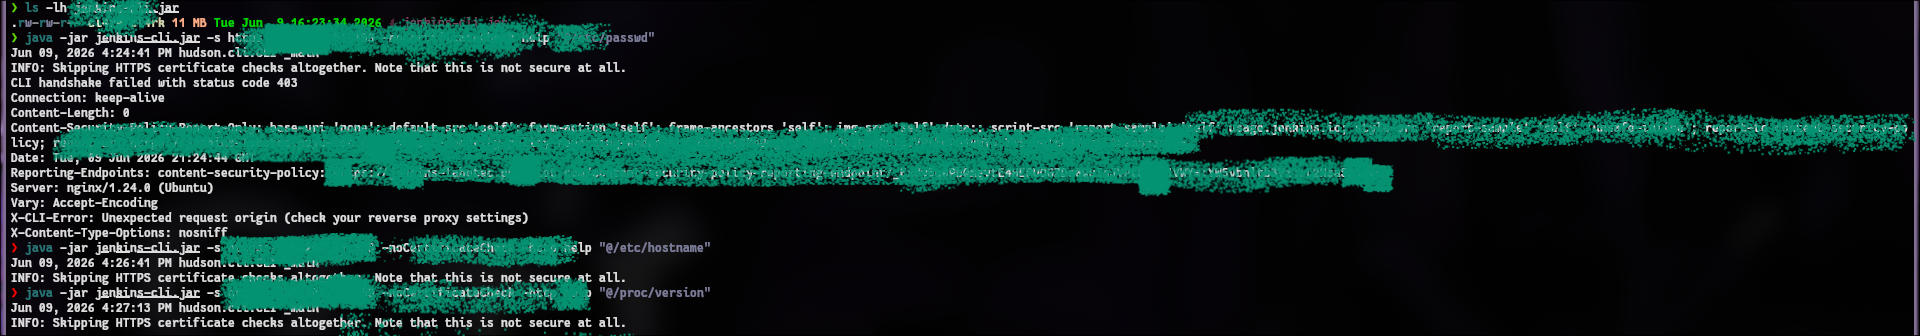
\includegraphics[width=0.82\textwidth]{../evidence/screenshots/199-jenkins-cli-cve-2024-23897-blocked.png}
\captionof*{figure}{\small\textcolor{textmuted}{CVE-2024-23897 bloqueado por el servidor}}
\end{center}

\textbf{Remediacion:}
\begin{itemize}[noitemsep]
  \item Mantener el proceso de actualizacion de Jenkins con revision periodica de CVEs.
  \item Deshabilitar el CLI remoto si no tiene uso operacional activo.
\end{itemize}
\end{tcolorbox}

\newpage

%% ============================================================
\section{Hallazgos --- Host B (HOST-B) --- Grafana / Laravel}
%% ============================================================

Servicios principales: Grafana (puerto 3000), Laravel (puerto 8080), phpMyAdmin (puerto 80).

\vspace{0.3cm}

%% ---- F-B-01 ----
\subsection{F-B-01 --- Grafana con credenciales por defecto}

\begin{tcolorbox}[colback=critical!6, colframe=critical, boxrule=1pt, arc=3pt,
  title={\textbf{F-B-01} \hfill \textbf{CRITICO $\cdot$ CVSS 9.8 $\cdot$ CWE-1188}},
  fonttitle=\bfseries\color{white}, coltitle=white, colbacktitle=critical, breakable]

\textbf{Host:} \texttt{HOST-B:3000}\\[4pt]

\textbf{Descripcion:}
El panel de administracion de Grafana acepta las credenciales por defecto
\texttt{admin:admin}. El acceso es inmediato, sin requerir ninguna tecnica
adicional. Una vez dentro, se obtuvo control administrativo completo:
visualizacion de dashboards de produccion, acceso a la configuracion de
datasources y posibilidad de modificar alertas activas del sistema GPS.

\begin{lstlisting}
curl -u admin:admin http://HOST-B:3000/api/org
# {"id":1,"name":"Main Org.","address":{}}

curl -sk http://HOST-B:3000/api/datasources -u admin:admin | python3 -m json.tool
# [{"type":"postgres","url":"...","database":"[REDACTED]",...}]
\end{lstlisting}

\begin{center}
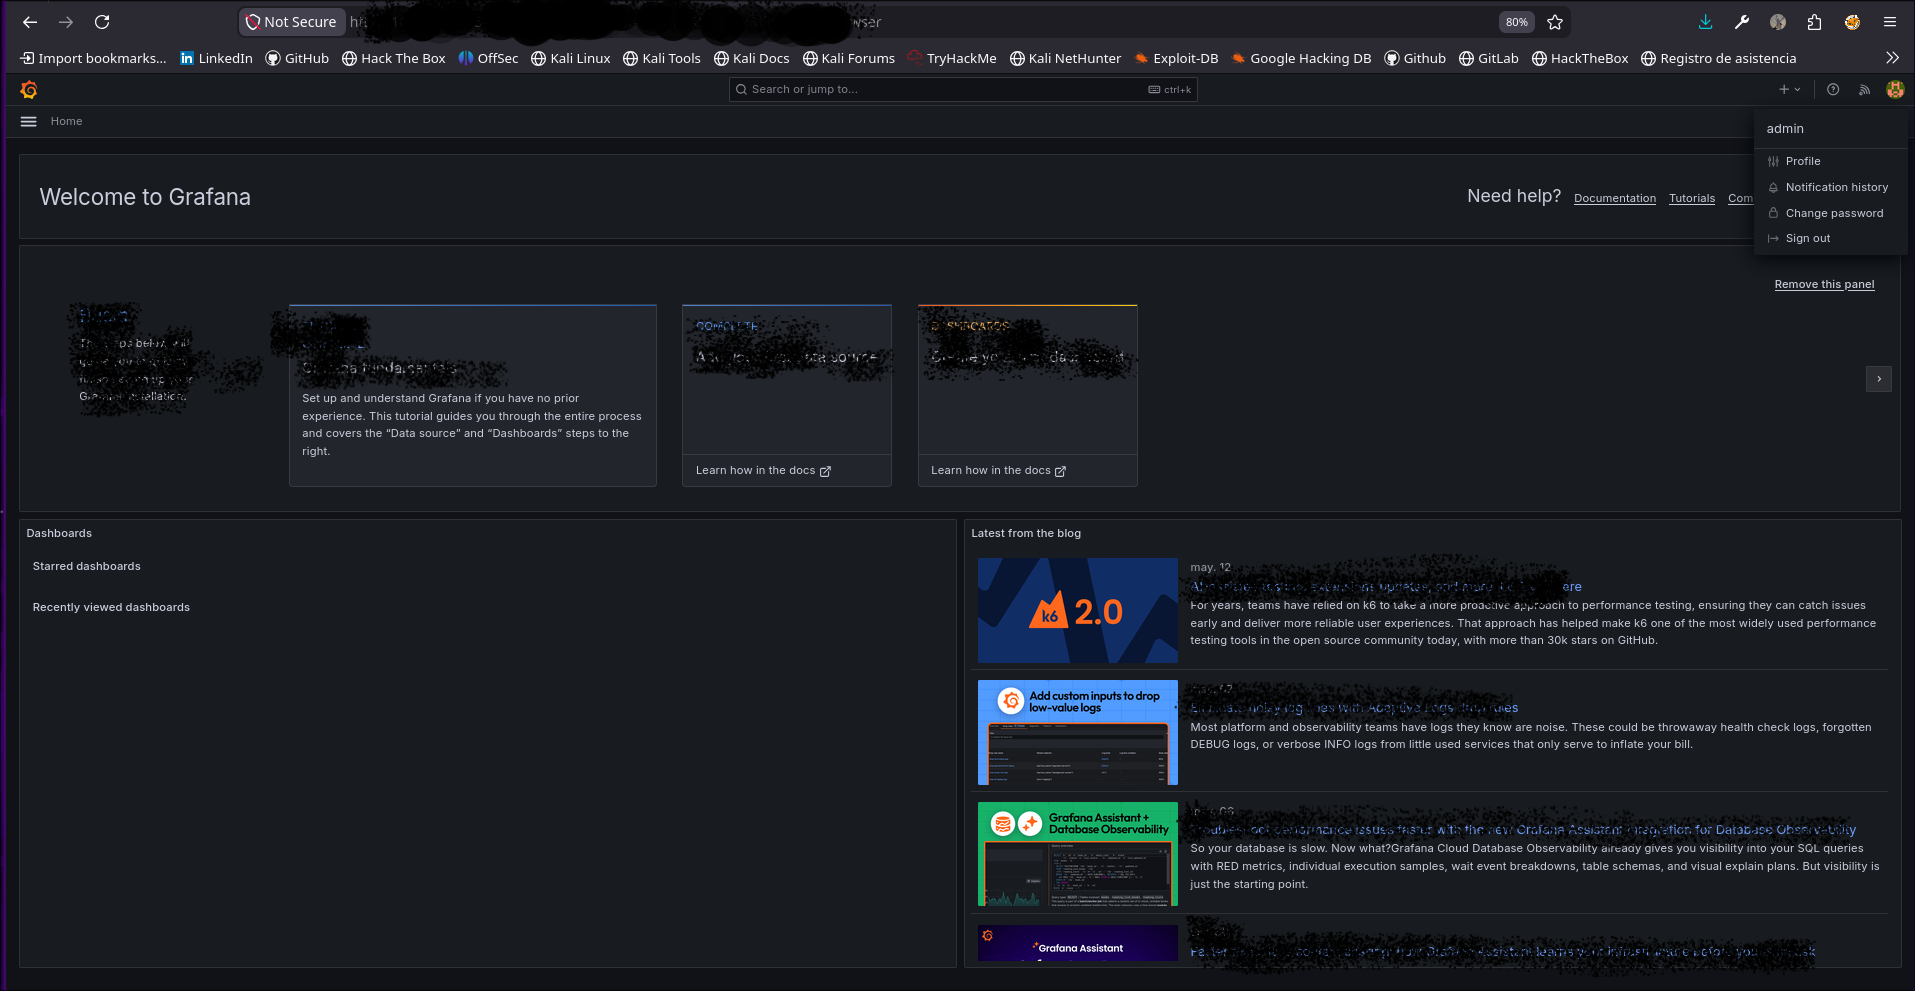
\includegraphics[width=0.82\textwidth]{../evidence/screenshots/234-grafana-login.png}
\captionof*{figure}{\small\textcolor{textmuted}{Acceso al panel de administracion con admin:admin}}
\end{center}

\begin{center}
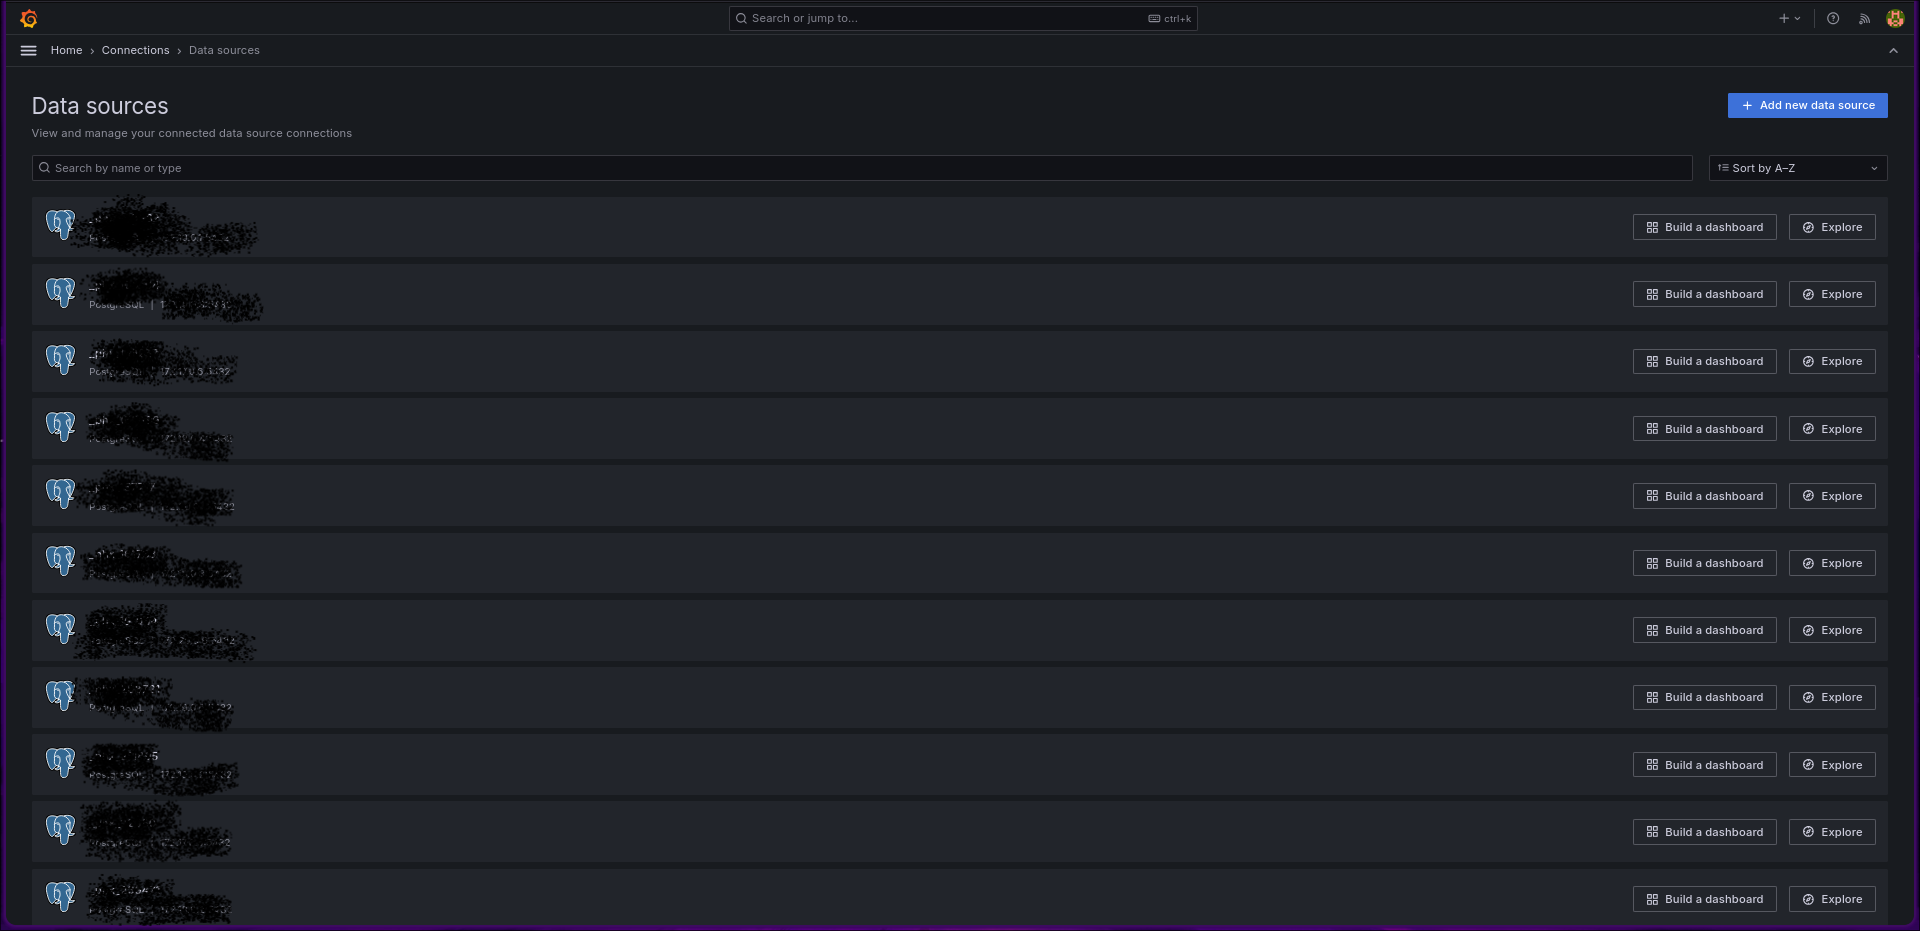
\includegraphics[width=0.82\textwidth]{../evidence/screenshots/234-grafana-datasources-postgresql.png}
\captionof*{figure}{\small\textcolor{textmuted}{Datasources PostgreSQL visibles tras el acceso}}
\end{center}

\textbf{Impacto:}
Acceso completo a la plataforma de monitoreo. Exposicion de configuracion
de bases de datos PostgreSQL internas. Un atacante puede leer metricas
de produccion, modificar dashboards y deshabilitar alertas de seguridad.

\textbf{Remediacion:}
\begin{itemize}[noitemsep]
  \item Cambiar la contrasena de \texttt{admin} de forma inmediata.
  \item Restringir el acceso al puerto 3000 a IPs autorizadas o red interna.
  \item Habilitar autenticacion multifactor en Grafana.
  \item Auditar los datasources configurados y reducir permisos a solo lectura.
\end{itemize}
\end{tcolorbox}

\vspace{0.4cm}

%% ---- F-B-02 ----
\subsection{F-B-02 --- Datasources PostgreSQL expuestos en Grafana}

\begin{tcolorbox}[colback=high!6, colframe=high, boxrule=1pt, arc=3pt,
  title={\textbf{F-B-02} \hfill \textbf{ALTO $\cdot$ CWE-200}},
  fonttitle=\bfseries\color{white}, coltitle=white, colbacktitle=high, breakable]

\textbf{Host:} \texttt{HOST-B:3000}\\[4pt]

\textbf{Descripcion:}
Tras el acceso con credenciales por defecto, los datasources de PostgreSQL
configurados en Grafana exponen nombres de bases de datos internas, hosts
y puertos. Las credenciales del datasource no fueron verificables directamente,
pero la exposicion de la cadena de conexion facilita ataques dirigidos
contra la base de datos.

\begin{center}
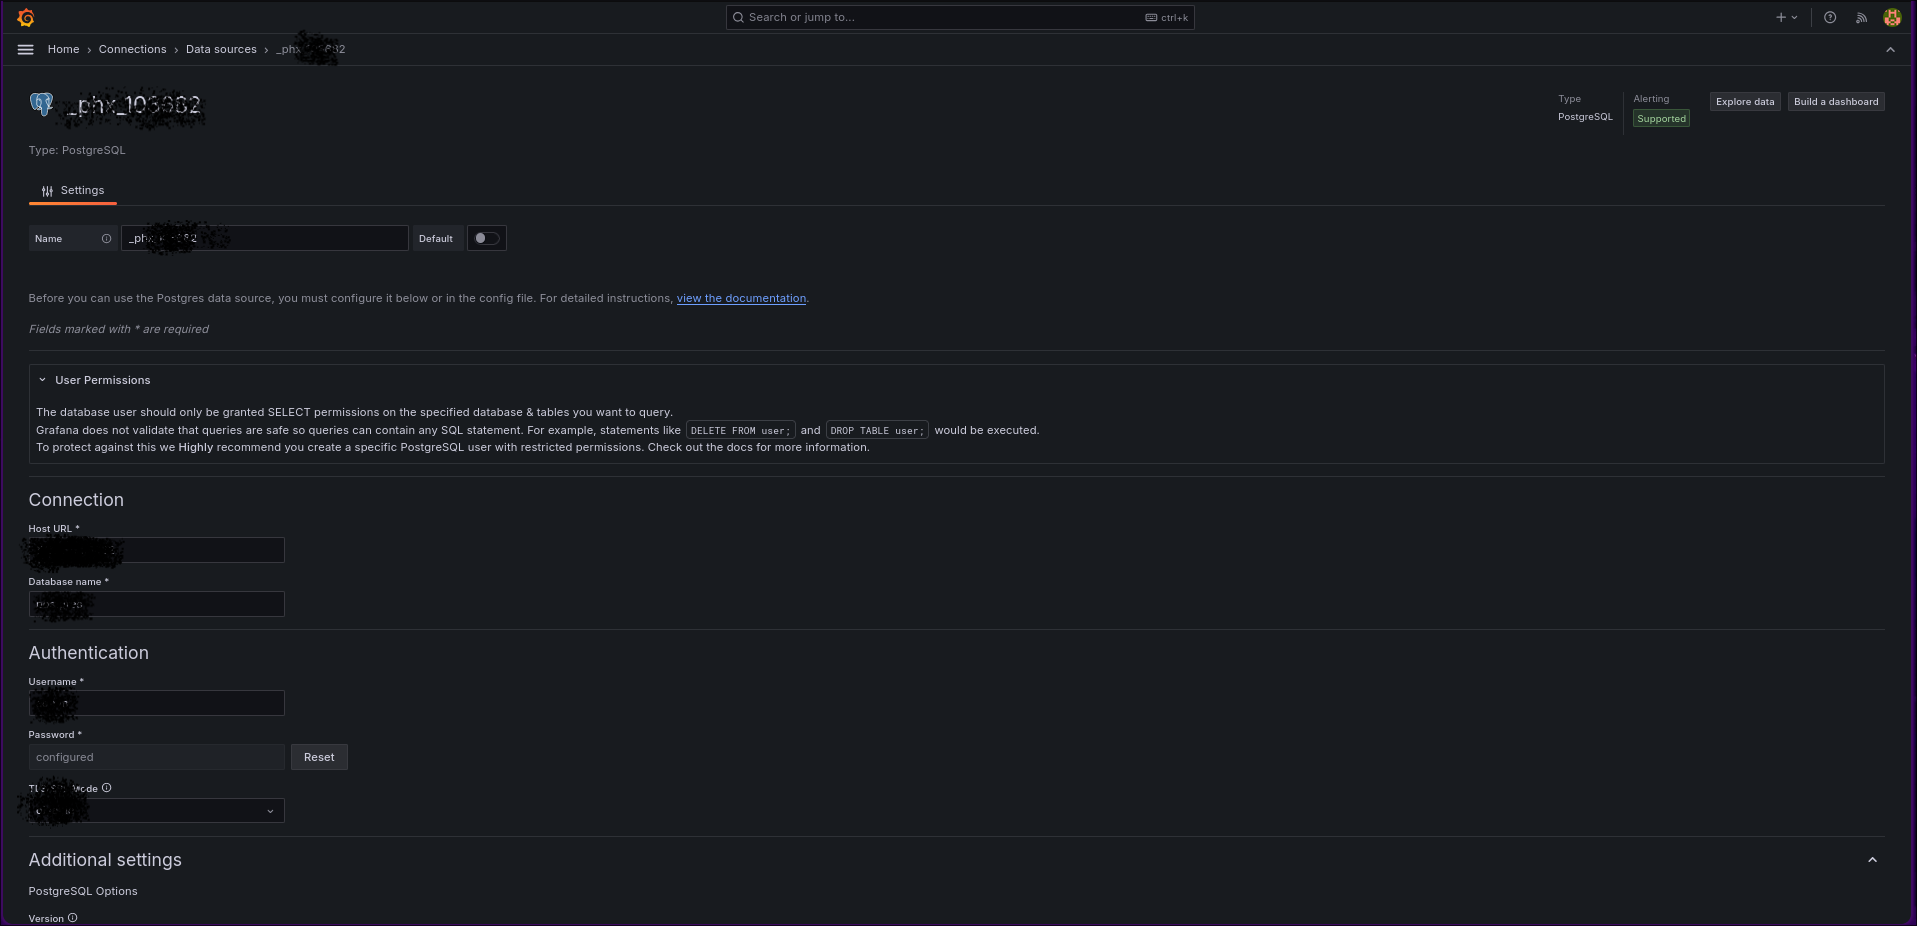
\includegraphics[width=0.82\textwidth]{../evidence/screenshots/234-grafana-postgresql.png}
\captionof*{figure}{\small\textcolor{textmuted}{Configuracion de datasource PostgreSQL expuesta}}
\end{center}

\begin{center}
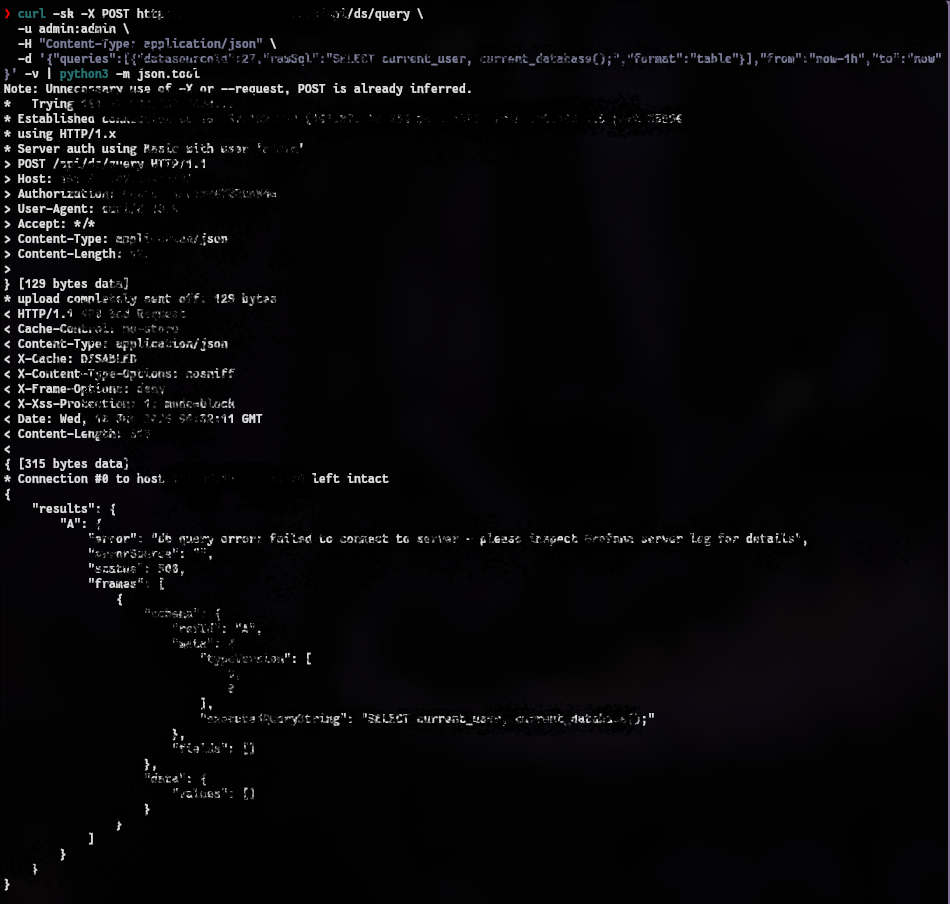
\includegraphics[width=0.82\textwidth]{../evidence/screenshots/234-grafana-query-failed.png}
\captionof*{figure}{\small\textcolor{textmuted}{Error de consulta revela nombre de base de datos interna}}
\end{center}

\textbf{Remediacion:}
\begin{itemize}[noitemsep]
  \item Usar cuentas de base de datos de solo lectura con permisos minimos para Grafana.
  \item Rotar las credenciales del datasource tras este hallazgo.
\end{itemize}
\end{tcolorbox}

\vspace{0.4cm}

%% ---- F-B-03 ----
\subsection{F-B-03 --- Laravel Debug Mode activo en produccion}

\begin{tcolorbox}[colback=high!6, colframe=high, boxrule=1pt, arc=3pt,
  title={\textbf{F-B-03} \hfill \textbf{ALTO $\cdot$ CWE-209}},
  fonttitle=\bfseries\color{white}, coltitle=white, colbacktitle=high, breakable]

\textbf{Host:} \texttt{HOST-B:8080}\\[4pt]

\textbf{Descripcion:}
La aplicacion Laravel tiene \texttt{APP\_DEBUG=true} en produccion. Los errores
HTTP devuelven stacktraces completos con rutas absolutas del servidor, versiones
exactas de dependencias y configuracion de conexion a base de datos. Esta
informacion reduce el tiempo de reconocimiento de un atacante y facilita
la identificacion de vectores de explotacion.

\begin{center}
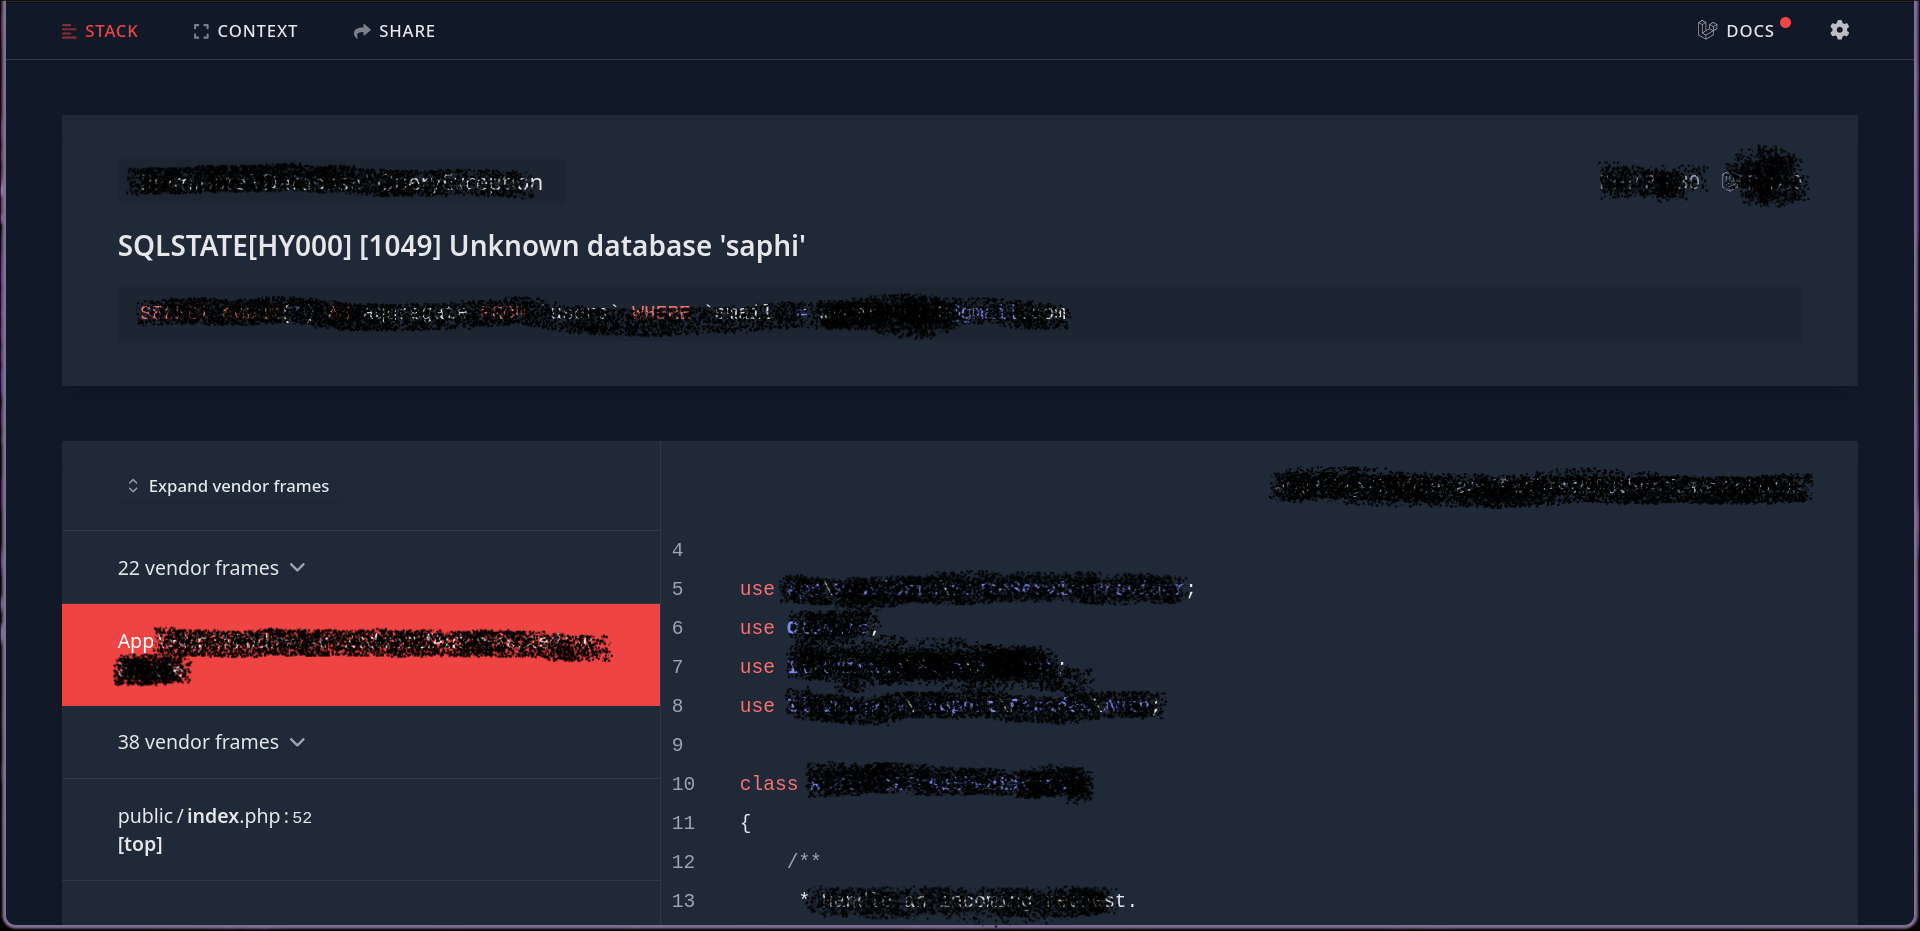
\includegraphics[width=0.82\textwidth]{../evidence/screenshots/234-laravel-debug-stacktrace-db-leak.png}
\captionof*{figure}{\small\textcolor{textmuted}{Stacktrace con rutas internas y configuracion de DB}}
\end{center}

\textbf{Remediacion:}
\begin{itemize}[noitemsep]
  \item Configurar \texttt{APP\_DEBUG=false} y \texttt{APP\_ENV=production} en el archivo \texttt{.env}.
  \item Implementar un handler de errores personalizado que no exponga informacion tecnica.
\end{itemize}
\end{tcolorbox}

\vspace{0.4cm}

%% ---- F-B-04 ----
\subsection{F-B-04 --- phpMyAdmin con Directory Listing habilitado}

\begin{tcolorbox}[colback=medium!10, colframe=medium, boxrule=1pt, arc=3pt,
  title={\textbf{F-B-04} \hfill \textbf{MEDIO $\cdot$ CWE-548}},
  fonttitle=\bfseries\color{white}, coltitle=white, colbacktitle=medium, breakable]

\textbf{Host:} \texttt{HOST-B:80}\\[4pt]

\textbf{Descripcion:}
Los directorios \texttt{/libraries/} y \texttt{/tmp/twig/} de phpMyAdmin tienen
el listado habilitado. Exponen la estructura interna de la aplicacion y las
versiones de las librerias instaladas, informacion util para identificar
componentes vulnerables.

\begin{center}
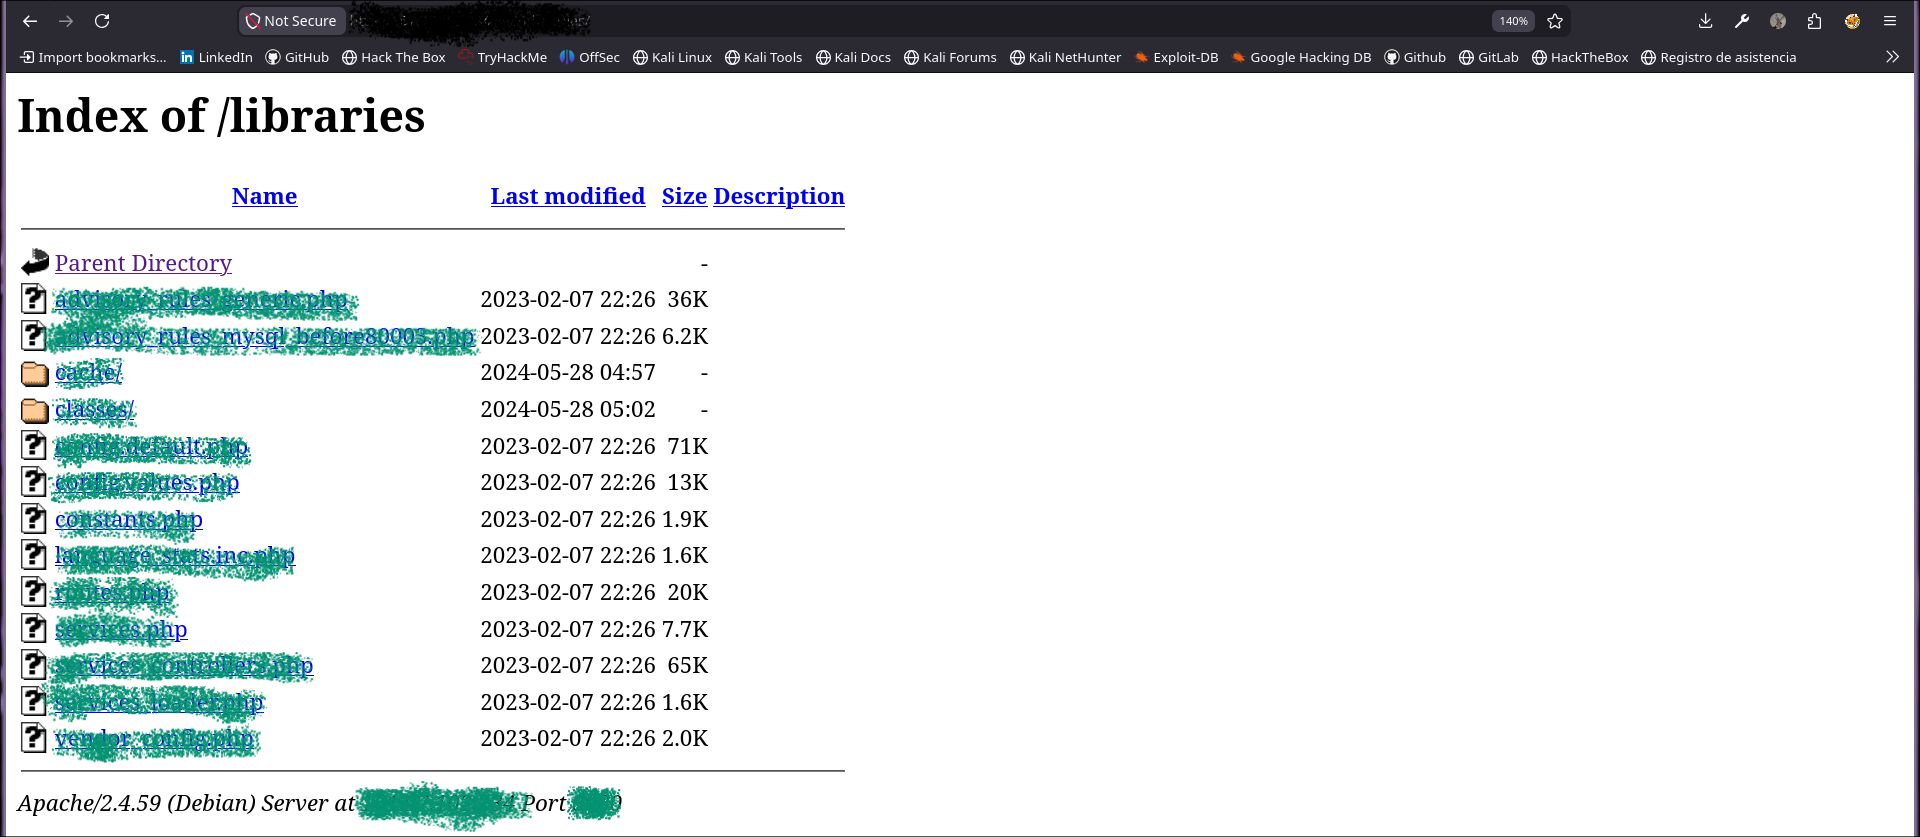
\includegraphics[width=0.82\textwidth]{../evidence/screenshots/234-phpmyadmin-libraries-directory.png}
\captionof*{figure}{\small\textcolor{textmuted}{Directory listing en /libraries/}}
\end{center}

\begin{center}
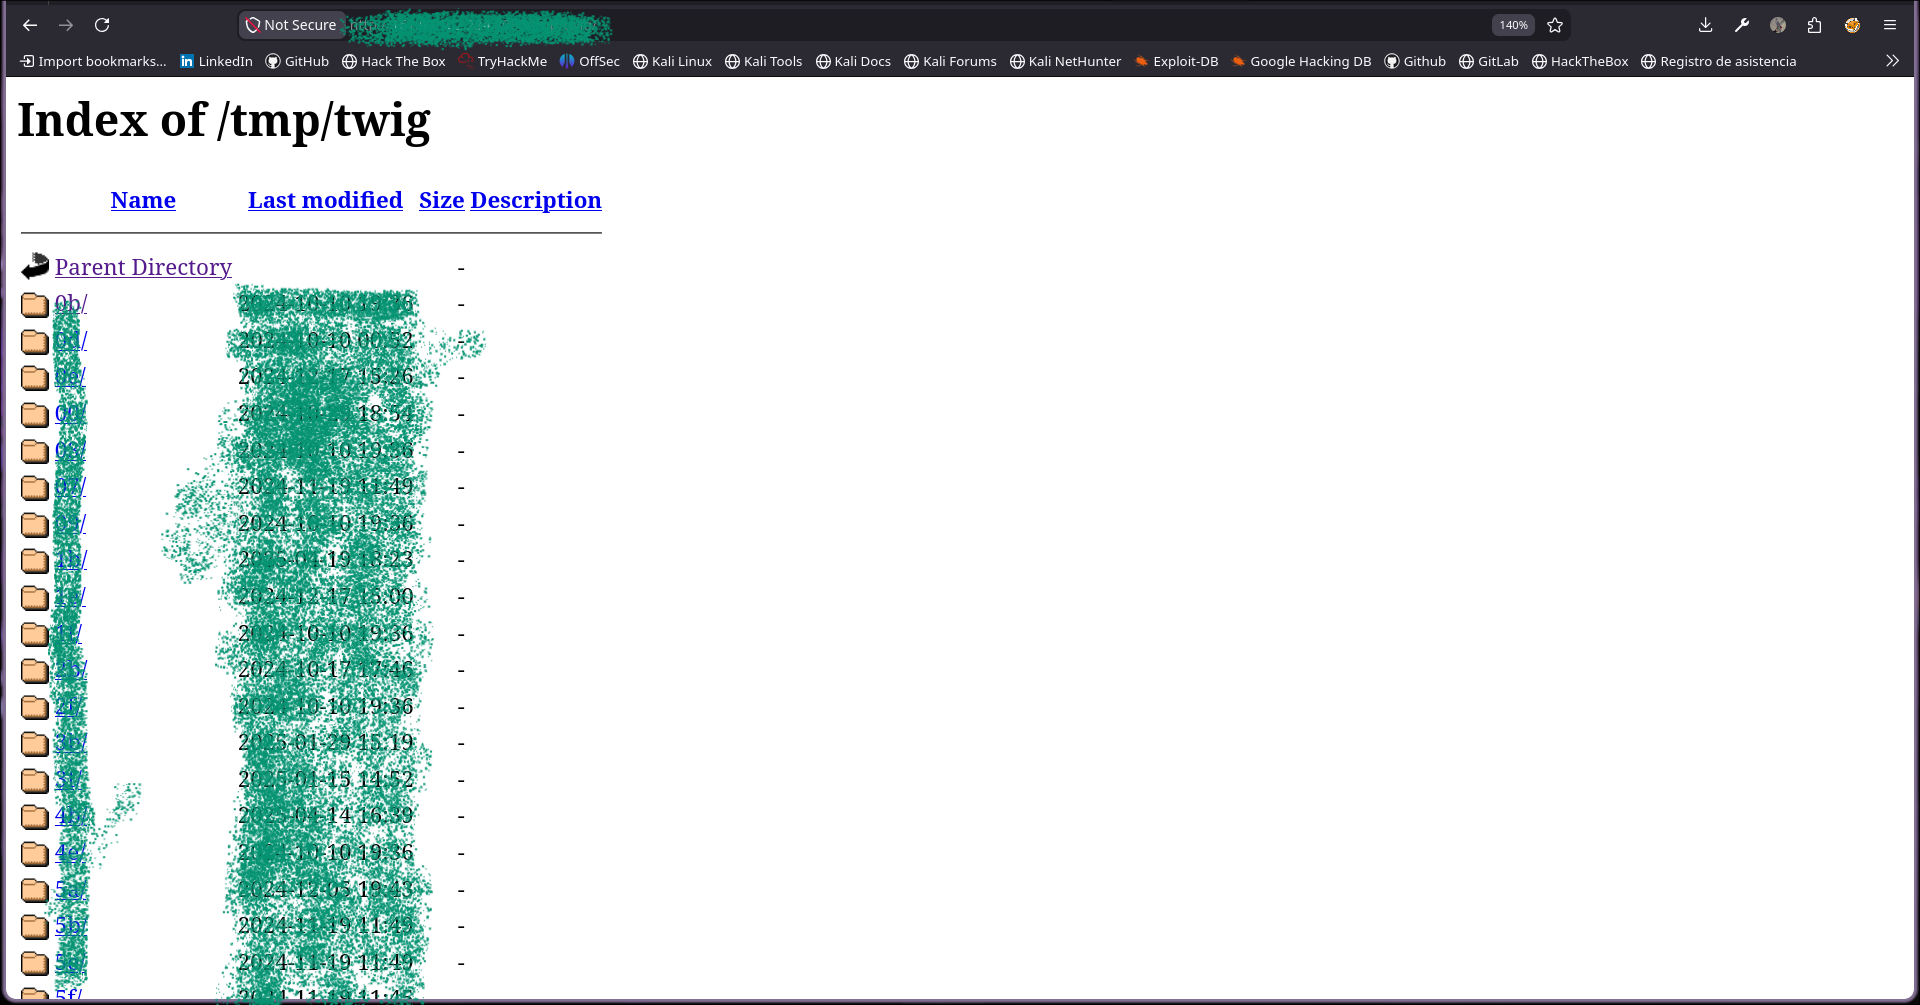
\includegraphics[width=0.82\textwidth]{../evidence/screenshots/234-phpmyadmin-tmp-twig-directory.png}
\captionof*{figure}{\small\textcolor{textmuted}{Directory listing en /tmp/twig/}}
\end{center}

\textbf{Remediacion:}
\begin{itemize}[noitemsep]
  \item Deshabilitar el listado de directorios: agregar \texttt{autoindex off;} en la configuracion de nginx.
\end{itemize}
\end{tcolorbox}

\vspace{0.4cm}

%% ---- F-B-05 ----
\subsection{F-B-05 --- MySQL expuesto publicamente en puerto 3306}

\begin{tcolorbox}[colback=high!6, colframe=high, boxrule=1pt, arc=3pt,
  title={\textbf{F-B-05} \hfill \textbf{ALTO $\cdot$ CWE-284}},
  fonttitle=\bfseries\color{white}, coltitle=white, colbacktitle=high, breakable]

\textbf{Host:} \texttt{HOST-B:3306}\\[4pt]

\textbf{Descripcion:}
El servicio MySQL es alcanzable directamente desde internet. El acceso como
\texttt{root} fue denegado, pero el puerto expuesto amplia la superficie de
ataque: permite bruteforce de otros usuarios, explotacion de vulnerabilidades
del motor y extraccion de informacion del banner de MySQL.

\begin{lstlisting}
mysql -h HOST-B -u root --password="" --skip-ssl
# ERROR 1130 (HY000): Host '...' is not allowed to connect
\end{lstlisting}

\begin{center}
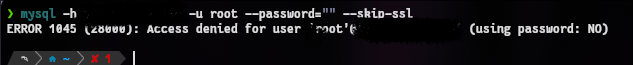
\includegraphics[width=0.82\textwidth]{../evidence/screenshots/234-mysql-root-access-denied.png}
\captionof*{figure}{\small\textcolor{textmuted}{Puerto 3306 accesible --- acceso root denegado}}
\end{center}

\textbf{Remediacion:}
\begin{itemize}[noitemsep]
  \item Restringir el puerto 3306 a conexiones locales o de red interna mediante firewall.
  \item Nunca exponer motores de base de datos directamente a internet.
\end{itemize}
\end{tcolorbox}

\newpage

%% ============================================================
\section{Hallazgos --- Host C (HOST-C) --- GPS Platform}
%% ============================================================

Servicios principales: Wiki.js (8080), Spring Boot (4300, 4305), MySQL (3306),
SSH (22), nginx. Sistema operativo confirmado: Ubuntu 24.04.4 LTS.
Proveedor: [REDACTED]. Recursos: 12 vCPU, 48 GB RAM, 250 GB NVMe.

\vspace{0.3cm}

%% ---- F-C-01 ----
\subsection{F-C-01 --- Wiki.js publica sin autenticacion}

\begin{tcolorbox}[colback=critical!6, colframe=critical, boxrule=1pt, arc=3pt,
  title={\textbf{F-C-01} \hfill \textbf{CRITICO $\cdot$ CVSS 9.1 $\cdot$ CWE-200}},
  fonttitle=\bfseries\color{white}, coltitle=white, colbacktitle=critical, breakable]

\textbf{Host:} \texttt{HOST-C:8080}\\[4pt]

\textbf{Descripcion:}
La instancia de Wiki.js es accesible sin autenticacion desde internet. Contiene
la documentacion tecnica completa del sistema GPS IoT: arquitectura de
microservicios, stack tecnologico, scripts de acceso a produccion, configuracion
de servicios externos y datos de los desarrolladores internos.

Informacion critica identificada en la wiki:
\begin{itemize}[noitemsep]
  \item Stack completo: Java 17, Spring Boot 3.3.4+, PostgreSQL, Redis, MongoDB, Kafka.
  \item Script \texttt{tunnels.sh} con acceso SSH como \texttt{root} al servidor de produccion.
  \item Configuracion de servicios externos: Twilio, SendGrid, Firebase.
  \item Topicos Kafka internos y contratos de mensajeria.
  \item Modelo de dominio completo: User, Device, Position, Vehicle.
  \item Recursos del servidor: IP publica, 12 vCPU, 48 GB RAM.
  \item Usuarios internos del equipo: Administrator, [REDACTED], [REDACTED].
\end{itemize}

\begin{center}
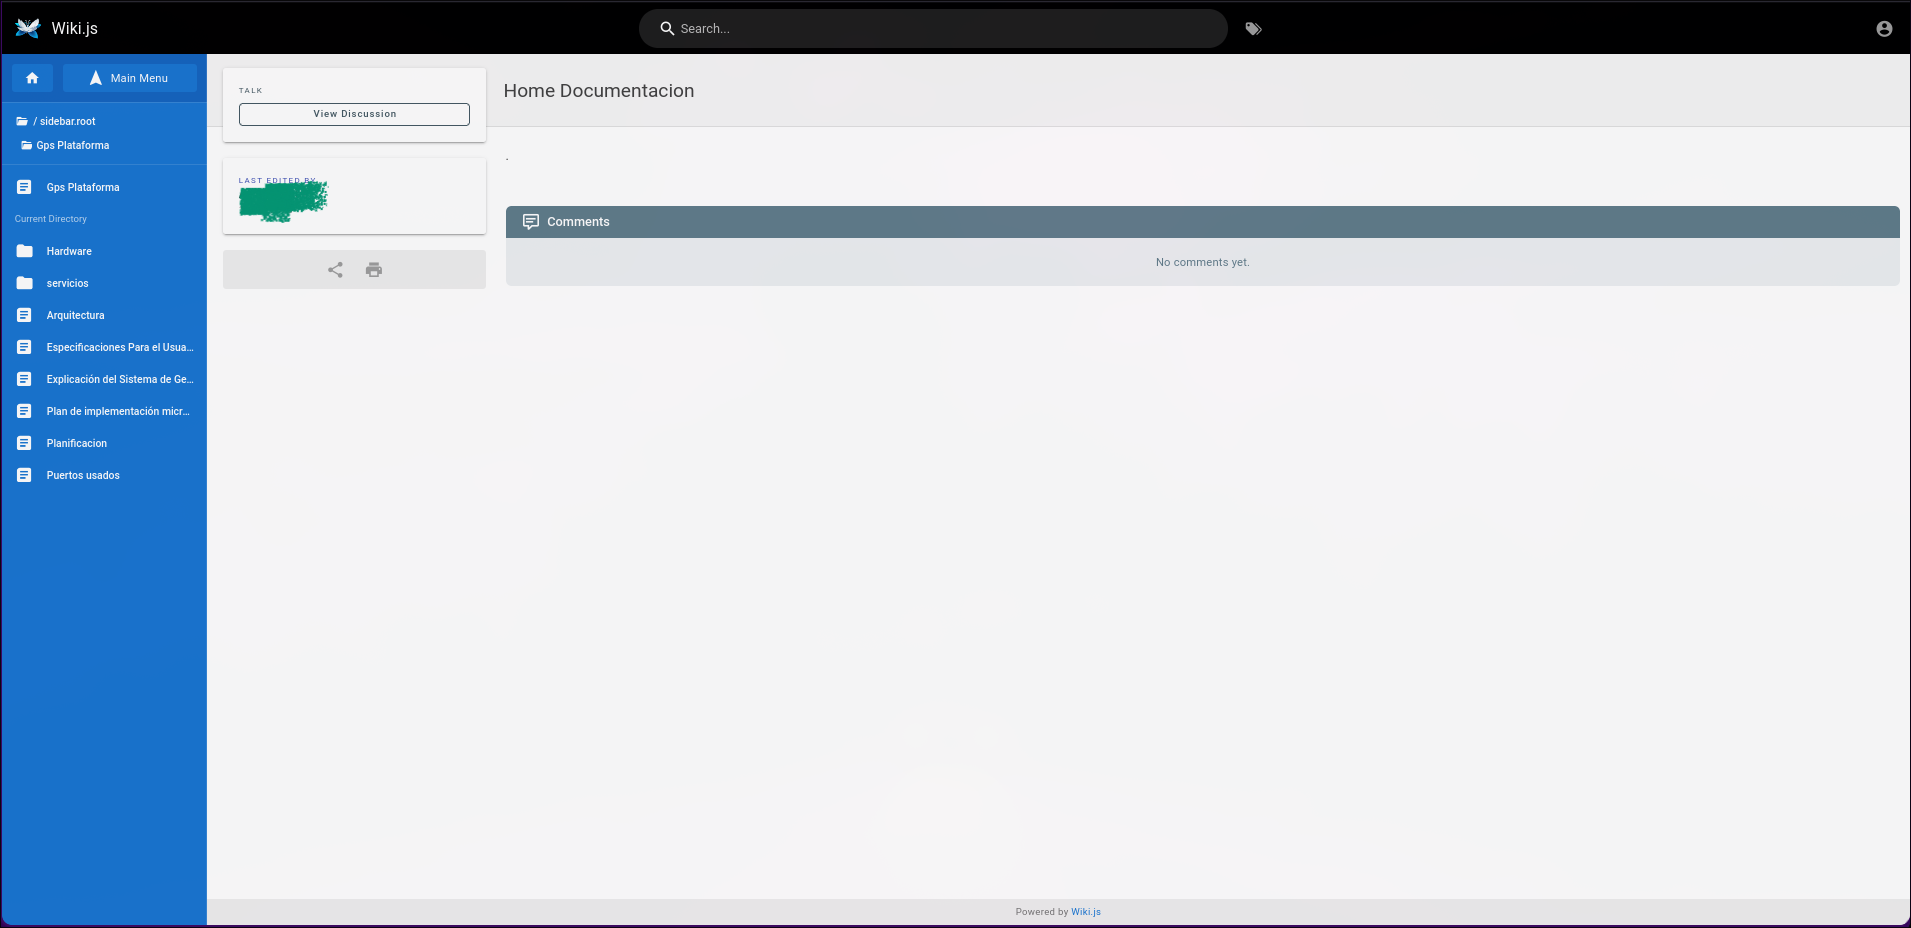
\includegraphics[width=0.82\textwidth]{../evidence/screenshots/100-wikijs-dasboard.png}
\captionof*{figure}{\small\textcolor{textmuted}{Wiki.js accesible sin autenticacion --- pagina principal}}
\end{center}

\begin{center}
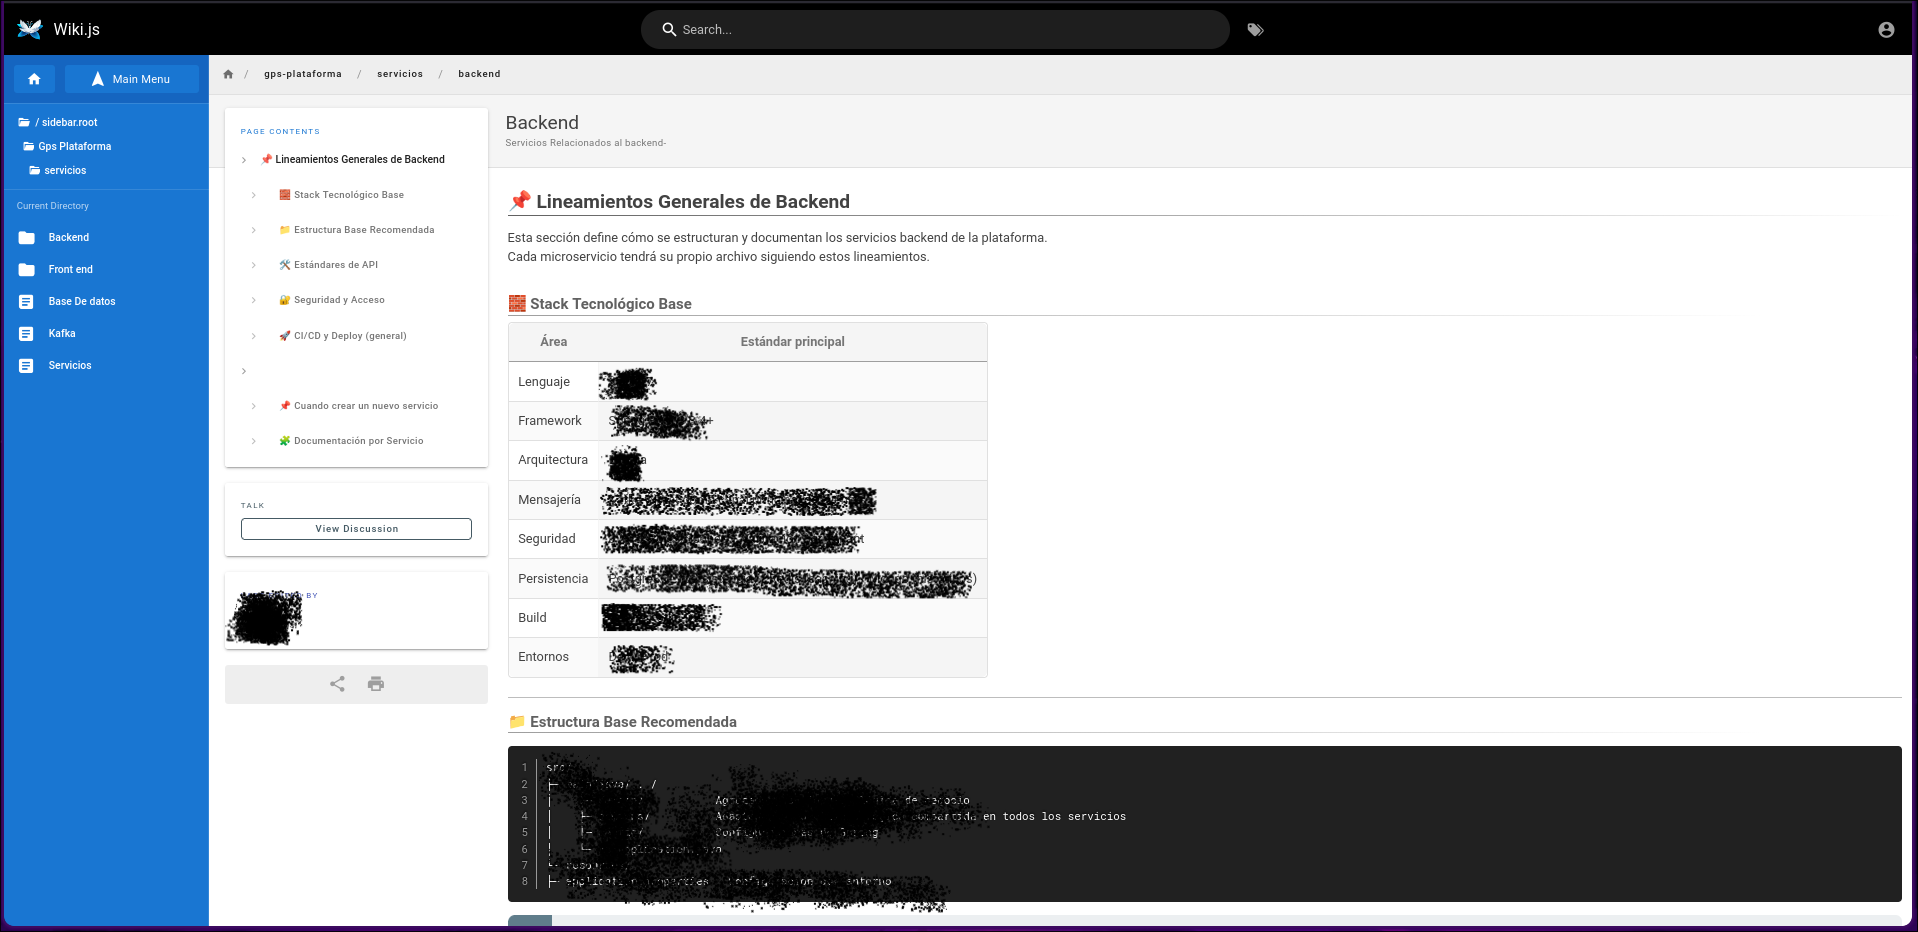
\includegraphics[width=0.82\textwidth]{../evidence/screenshots/100-wikijs-backend-lineamientos-gabo.png}
\captionof*{figure}{\small\textcolor{textmuted}{Documentacion interna de backend con tunnels.sh expuesto}}
\end{center}

\textbf{Impacto:}
Un atacante externo obtiene un mapa completo de la infraestructura antes de
ejecutar cualquier ataque. La informacion disponible permite planificar
ataques dirigidos contra cada componente del sistema sin necesidad de
reconocimiento adicional.

\textbf{Remediacion:}
\begin{itemize}[noitemsep]
  \item Habilitar autenticacion obligatoria en Wiki.js de forma inmediata.
  \item Mover la wiki a una red interna o protegerla con VPN.
  \item Auditar y rotar todas las credenciales y tokens mencionados en la wiki.
\end{itemize}
\end{tcolorbox}

\vspace{0.4cm}

%% ---- F-C-02 ----
\subsection{F-C-02 --- tunnels.sh con acceso root SSH expuesto}

\begin{tcolorbox}[colback=critical!6, colframe=critical, boxrule=1pt, arc=3pt,
  title={\textbf{F-C-02} \hfill \textbf{CRITICO $\cdot$ CVSS 9.8 $\cdot$ CWE-312}},
  fonttitle=\bfseries\color{white}, coltitle=white, colbacktitle=critical, breakable]

\textbf{Host:} \texttt{HOST-C:8080} (Wiki.js)\\[4pt]

\textbf{Descripcion:}
La wiki expone publicamente el script \texttt{tunnels.sh} utilizado por el
equipo de desarrollo para conectarse al servidor de produccion. El script
revela el usuario de acceso (\texttt{root}), la IP publica del servidor y
el mapa completo de puertos internos tuneados via SSH.

\begin{lstlisting}
#!/bin/bash
# Script para abrir tuneles SSH
ssh -N \
  -L 9092:localhost:9092 \  # Kafka
  -L 4350:localhost:4350 \  # Core Service
  -L 4305:localhost:4305 \  # TCP Server
  -L 4315:localhost:4315 \  # WebSocket Service
  -L 5432:localhost:5432 \  # Base de datos
  root@HOST-C
\end{lstlisting}

\begin{center}
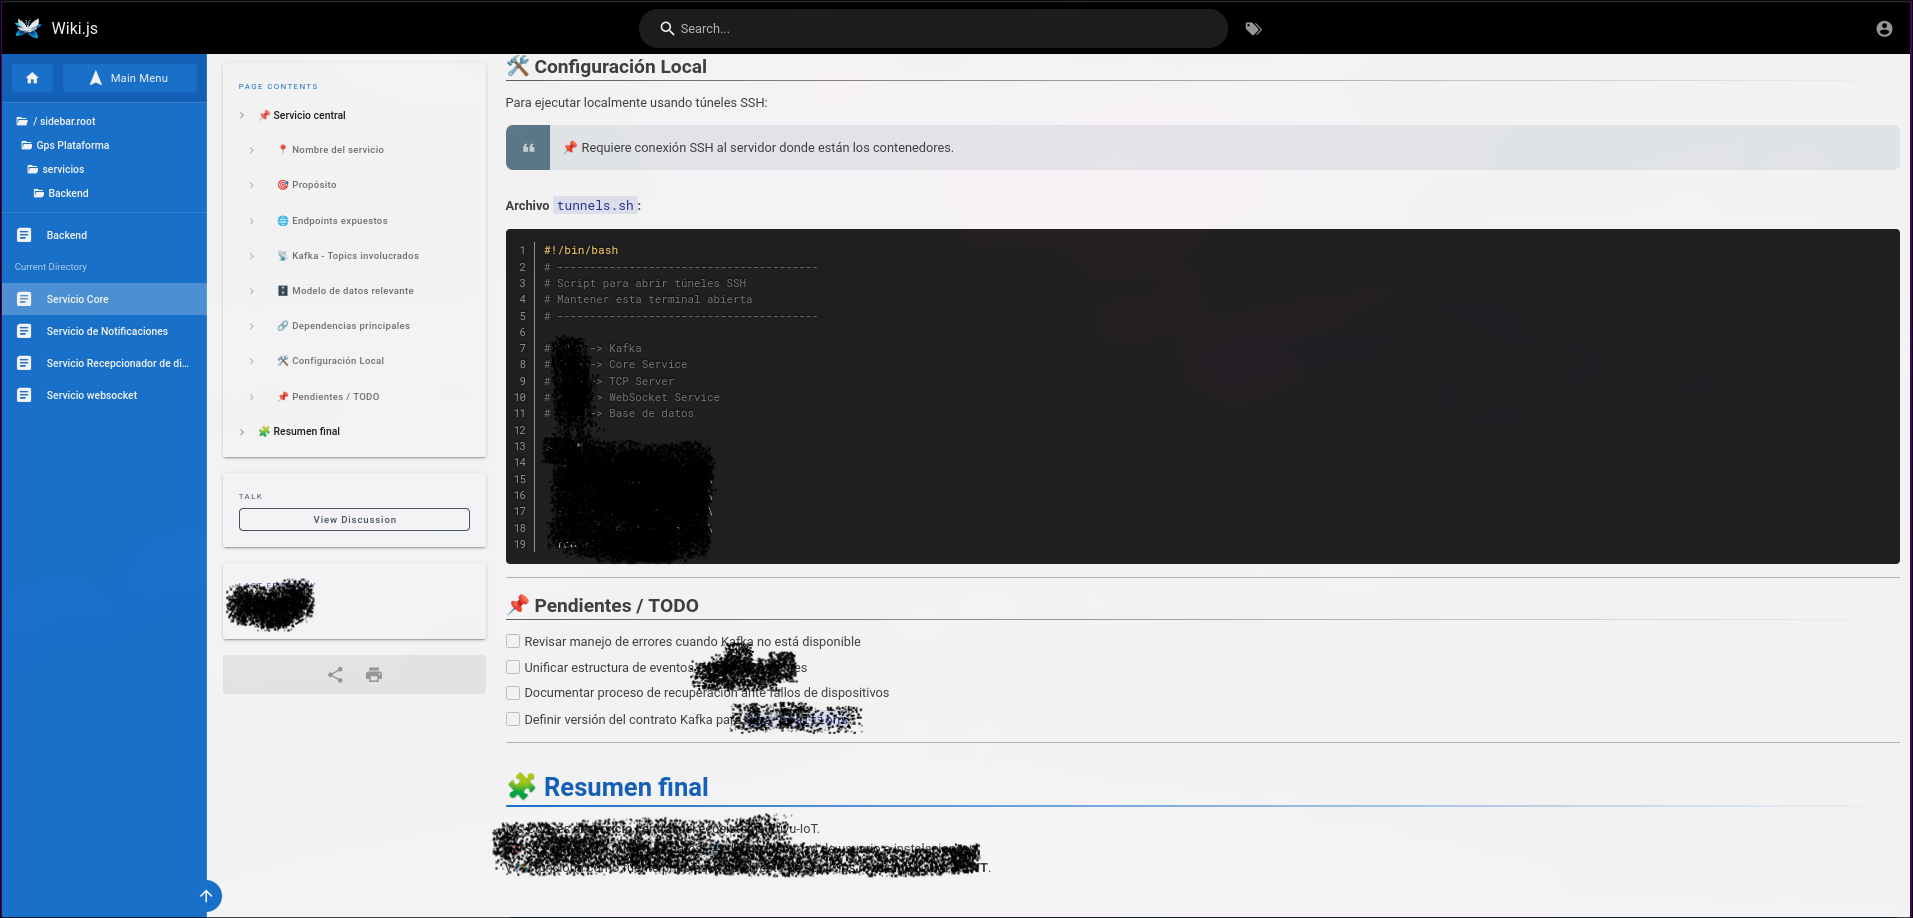
\includegraphics[width=0.82\textwidth]{../evidence/screenshots/100-wikijs-backend-tunnel.png}
\captionof*{figure}{\small\textcolor{textmuted}{Script tunnels.sh con root y puertos internos expuesto en la wiki}}
\end{center}

\textbf{Impacto:}
Con este script un atacante sabe exactamente donde atacar: usuario \texttt{root},
IP \texttt{HOST-C}, acceso SSH. Combinado con la ausencia de
proteccion anti-bruteforce (F-C-08), el vector hacia el compromiso total
del servidor esta documentado publicamente.

\textbf{Remediacion:}
\begin{itemize}[noitemsep]
  \item Eliminar \texttt{tunnels.sh} de la wiki inmediatamente.
  \item Deshabilitar login SSH como \texttt{root}: \texttt{PermitRootLogin no}.
  \item Crear usuarios de deploy sin privilegios de root.
  \item Implementar autenticacion SSH exclusivamente por clave publica.
\end{itemize}
\end{tcolorbox}

\vspace{0.4cm}

%% ---- F-C-03 ----
\subsection{F-C-03 --- GraphQL Introspection habilitada sin autenticacion}

\begin{tcolorbox}[colback=medium!10, colframe=medium, boxrule=1pt, arc=3pt,
  title={\textbf{F-C-03} \hfill \textbf{MEDIO $\cdot$ CWE-200}},
  fonttitle=\bfseries\color{white}, coltitle=white, colbacktitle=medium, breakable]

\textbf{Host:} \texttt{HOST-C:8080/graphql}\\[4pt]

\textbf{Descripcion:}
El endpoint GraphQL de Wiki.js tiene la introspection habilitada sin
autenticacion. Expone el schema completo de la API incluyendo tipos, queries,
mutations y campos sensibles relacionados con autenticacion y gestion de usuarios.

Tipos criticos expuestos: \texttt{UserQuery}, \texttt{UserMutation},
\texttt{AuthenticationQuery}, \texttt{AuthenticationApiKey},
\texttt{SystemInfo}, \texttt{GroupQuery}, \texttt{StorageQuery}.

\begin{lstlisting}
curl -X POST http://HOST-C:8080/graphql \
  -H "Content-Type: application/json" \
  -d '{"query":"{__schema{types{name}}}"}'
# {"data":{"__schema":{"types":[{"name":"UserQuery"},...]}}}
\end{lstlisting}

\begin{center}
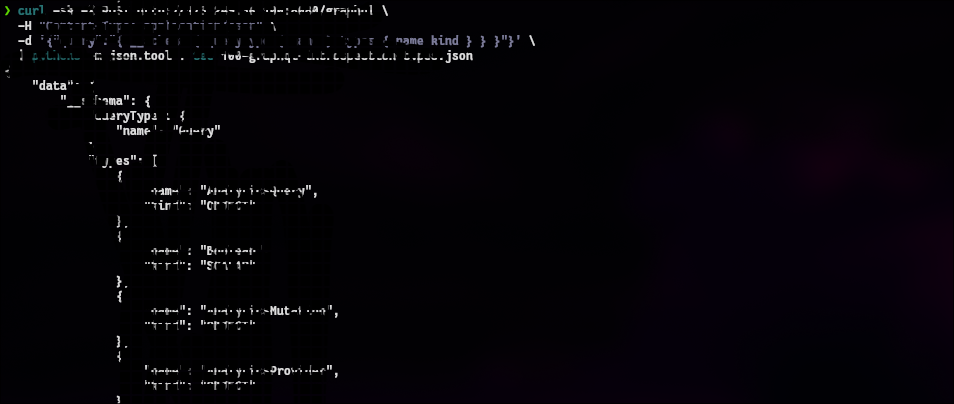
\includegraphics[width=0.82\textwidth]{../evidence/screenshots/100-graphql-introspection-types.png}
\captionof*{figure}{\small\textcolor{textmuted}{Schema GraphQL completo accesible sin autenticacion}}
\end{center}

\textbf{Remediacion:}
\begin{itemize}[noitemsep]
  \item Deshabilitar introspection en produccion: configurar \texttt{introspection: false} en Apollo Server.
\end{itemize}
\end{tcolorbox}

\vspace{0.4cm}

%% ---- F-C-04 ----
\subsection{F-C-04 --- GraphQL stacktrace con rutas internas}

\begin{tcolorbox}[colback=low!6, colframe=low, boxrule=1pt, arc=3pt,
  title={\textbf{F-C-04} \hfill \textbf{BAJO $\cdot$ CWE-209}},
  fonttitle=\bfseries\color{white}, coltitle=white, colbacktitle=low, breakable]

\textbf{Host:} \texttt{HOST-C:8080/graphql}\\[4pt]

\textbf{Descripcion:}
Los errores del endpoint GraphQL incluyen stacktraces con rutas absolutas
del servidor y estructura de \texttt{node\_modules}.

\begin{lstlisting}
# Ejemplo de ruta expuesta:
/wiki/server/graph/directives/auth.js:47:17
/wiki/node_modules/apollo-server-core/dist/utils/...
/wiki/node_modules/graphql/execution/execute.js
\end{lstlisting}

\begin{center}
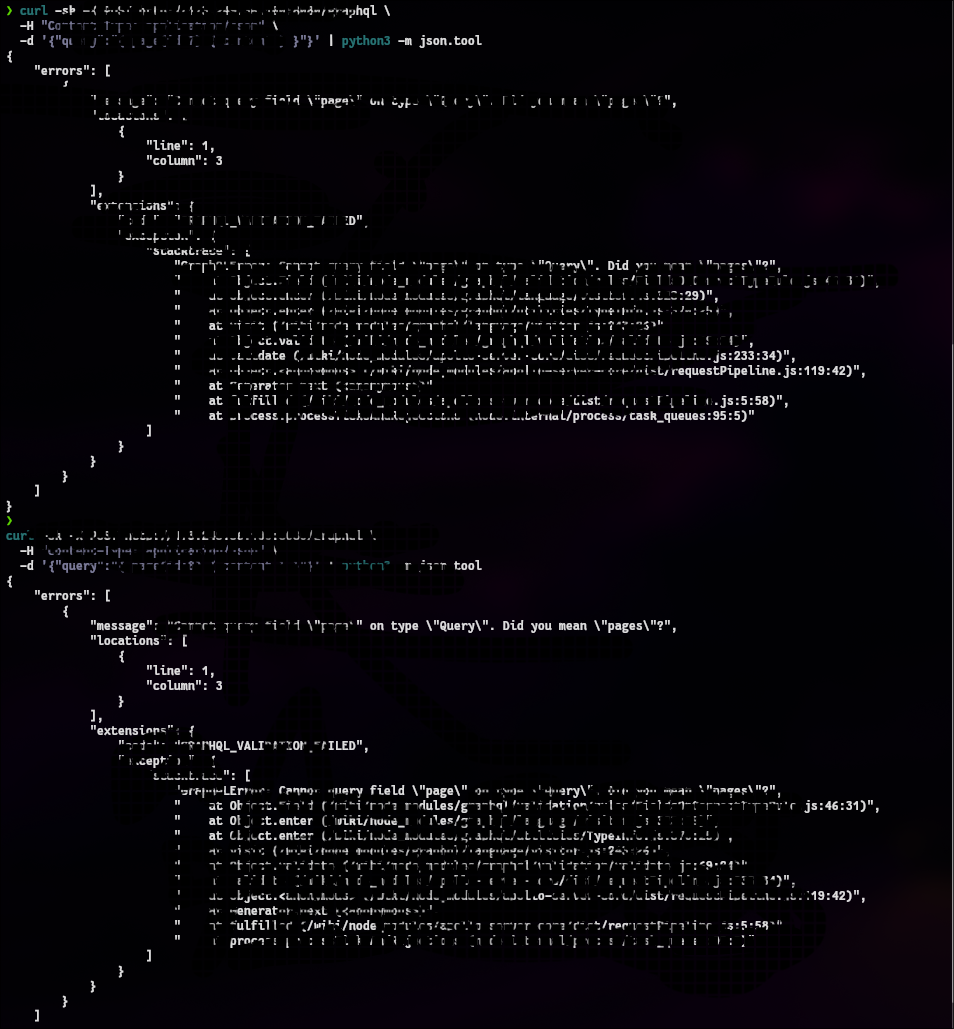
\includegraphics[width=0.82\textwidth]{../evidence/screenshots/100-graphql-stacktrace-1.png}
\captionof*{figure}{\small\textcolor{textmuted}{Stacktrace con rutas absolutas del servidor}}
\end{center}

\begin{center}
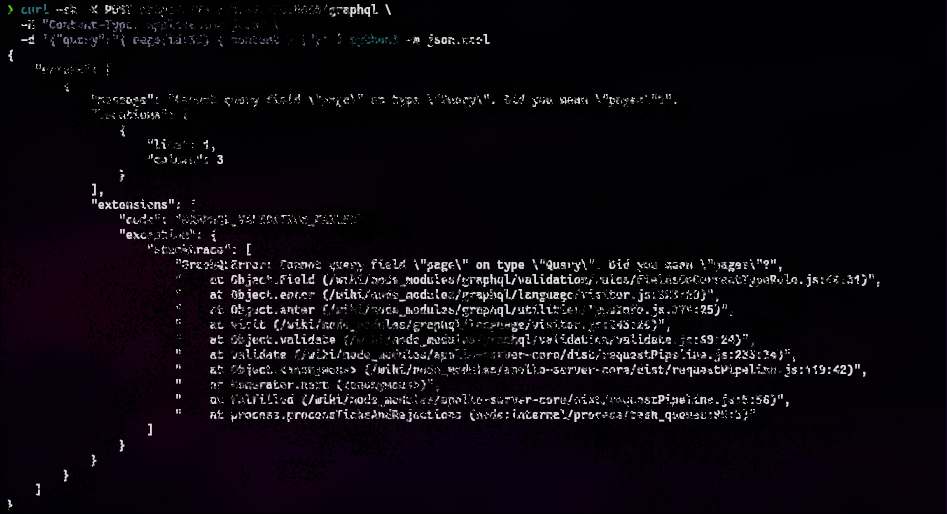
\includegraphics[width=0.82\textwidth]{../evidence/screenshots/100-graphql-stacktrace-2.png}
\captionof*{figure}{\small\textcolor{textmuted}{Stacktrace adicional con estructura de node\_modules}}
\end{center}

\textbf{Remediacion:}
\begin{itemize}[noitemsep]
  \item Sanitizar errores usando \texttt{formatError} en Apollo Server para produccion.
\end{itemize}
\end{tcolorbox}

\vspace{0.4cm}

%% ---- F-C-05 ----
\subsection{F-C-05 --- Spring Boot Actuator sin autenticacion}

\begin{tcolorbox}[colback=medium!10, colframe=medium, boxrule=1pt, arc=3pt,
  title={\textbf{F-C-05} \hfill \textbf{MEDIO $\cdot$ CWE-200}},
  fonttitle=\bfseries\color{white}, coltitle=white, colbacktitle=medium, breakable]

\textbf{Hosts:} \texttt{HOST-C:4300} y \texttt{HOST-C:4305}\\[4pt]

\textbf{Descripcion:}
Los endpoints de Spring Boot Actuator son accesibles sin autenticacion.
El endpoint \texttt{/actuator/prometheus} expone IPs internas de los
contenedores Docker, configuracion del pool de conexiones y metricas
del sistema y JVM.

Datos criticos expuestos:
\begin{itemize}[noitemsep]
  \item Puerto 4300: Redis interno en \texttt{172.21.0.20:6379}, HikariPool-1 con 50 conexiones minimas.
  \item Puerto 4305: Redis interno en \texttt{172.21.0.3:6379}, 122 conexiones TCP activas.
\end{itemize}

\begin{center}
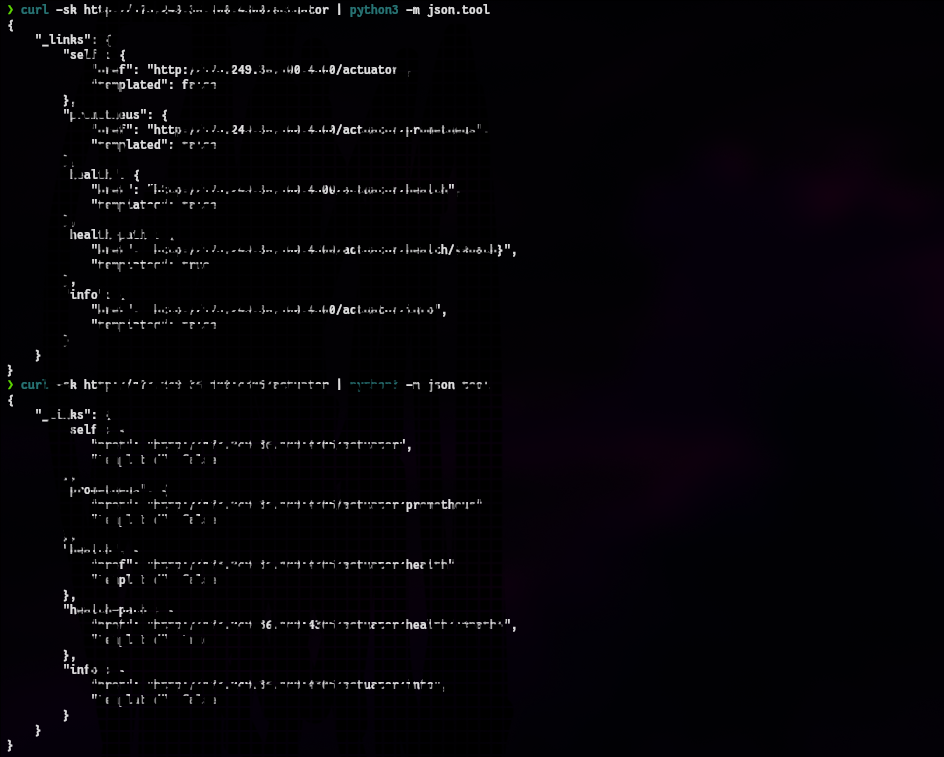
\includegraphics[width=0.82\textwidth]{../evidence/screenshots/100-actuator-4300-4305-open.png}
\captionof*{figure}{\small\textcolor{textmuted}{Endpoints Actuator accesibles en puertos 4300 y 4305}}
\end{center}

\begin{center}
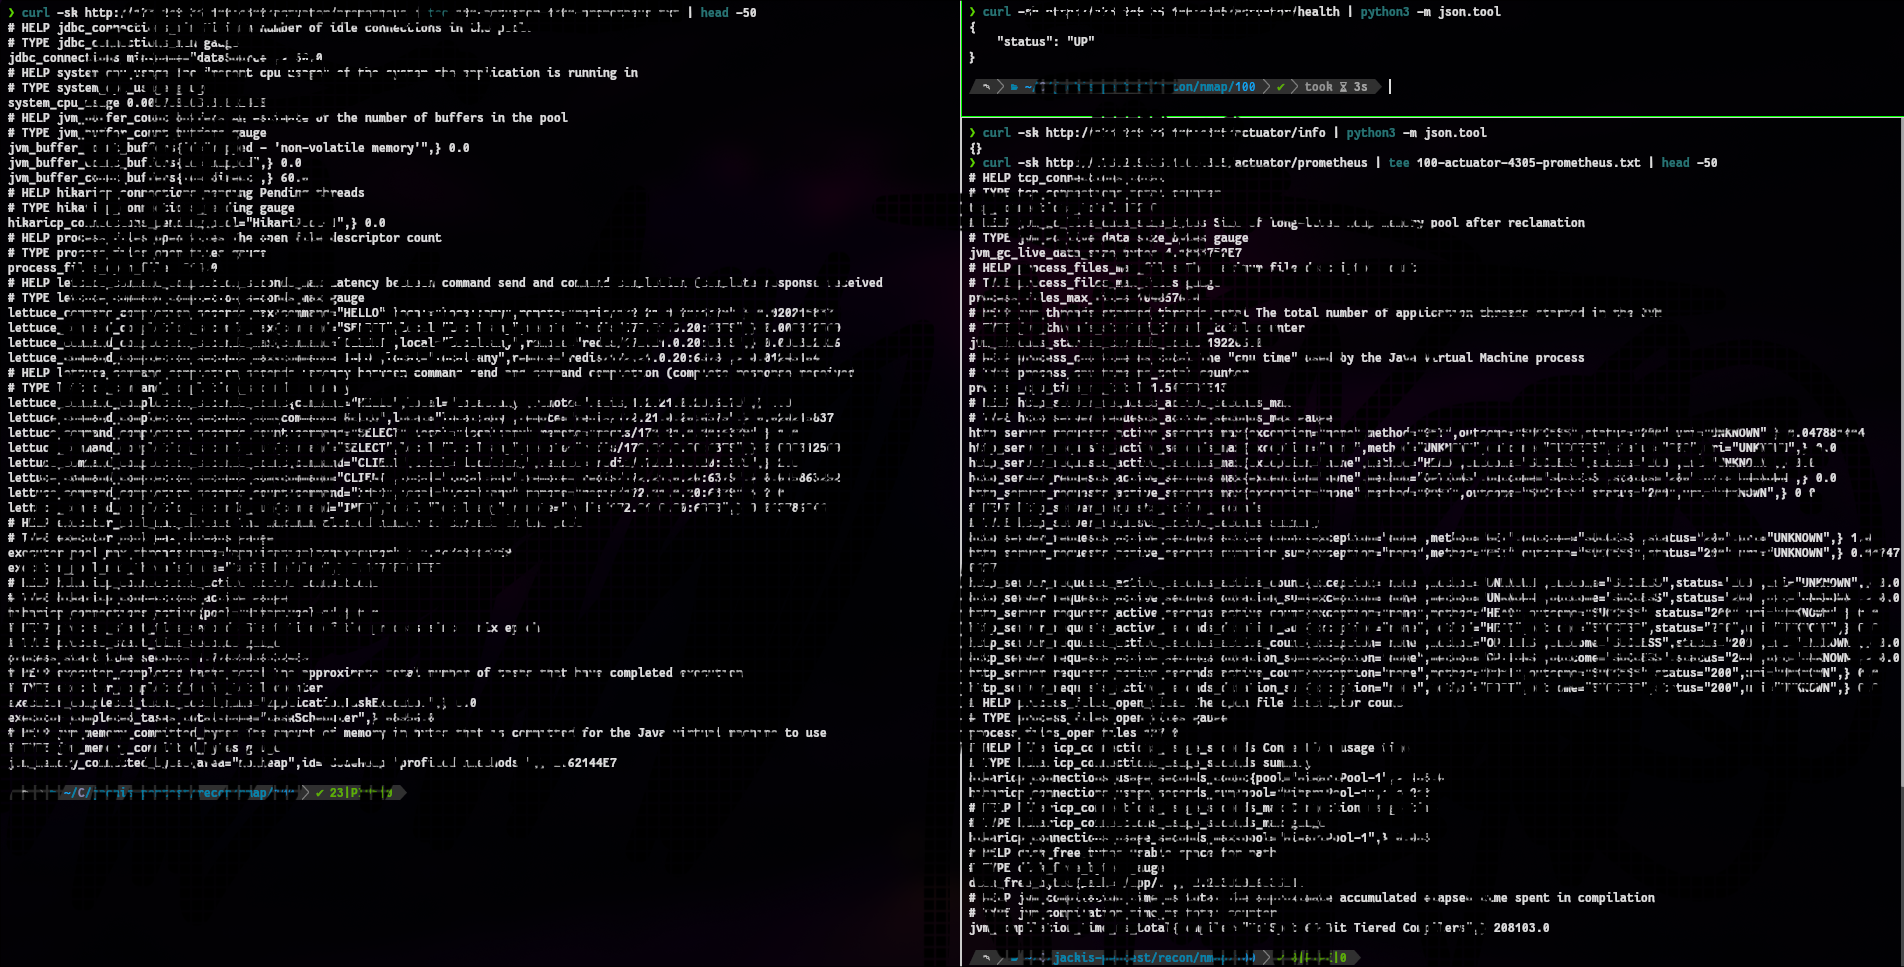
\includegraphics[width=0.82\textwidth]{../evidence/screenshots/100-actuator-prometheus-redis-ips.png}
\captionof*{figure}{\small\textcolor{textmuted}{IPs internas de Redis expuestas via /actuator/prometheus}}
\end{center}

\begin{center}
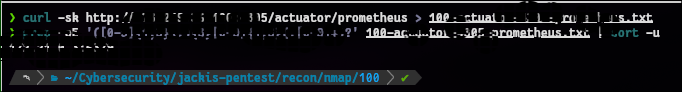
\includegraphics[width=0.82\textwidth]{../evidence/screenshots/100-actuator-4300-redis-172-21-0-20.png}
\captionof*{figure}{\small\textcolor{textmuted}{Redis 172.21.0.20:6379 expuesto en puerto 4300}}
\end{center}

\begin{center}
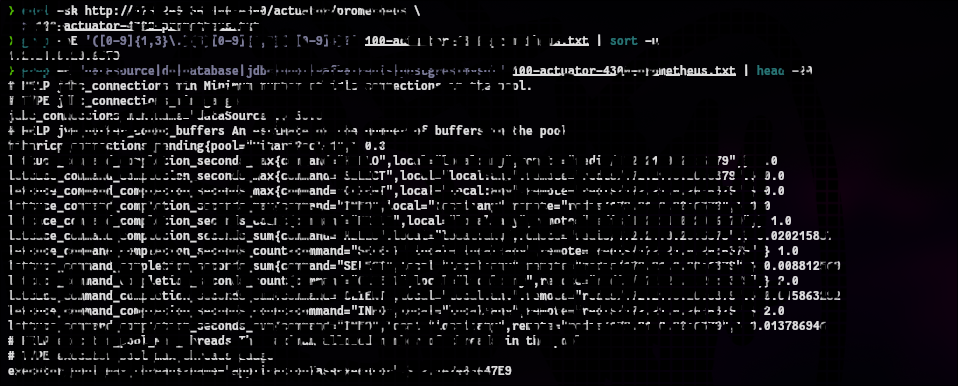
\includegraphics[width=0.82\textwidth]{../evidence/screenshots/100-actuator-4305-redis-172-21-0-3.png}
\captionof*{figure}{\small\textcolor{textmuted}{Redis 172.21.0.3:6379 expuesto en puerto 4305}}
\end{center}

\textbf{Remediacion:}
\begin{itemize}[noitemsep]
  \item Proteger los endpoints Actuator con Spring Security.
  \item Exponer unicamente \texttt{/actuator/health} si es necesario para monitoreo externo.
  \item Nunca exponer \texttt{/actuator/prometheus} o \texttt{/actuator/env} publicamente.
\end{itemize}
\end{tcolorbox}

\vspace{0.4cm}

%% ---- F-C-06 ----
\subsection{F-C-06 --- Spring Boot expone debugMessage en produccion}

\begin{tcolorbox}[colback=medium!10, colframe=medium, boxrule=1pt, arc=3pt,
  title={\textbf{F-C-06} \hfill \textbf{MEDIO $\cdot$ CWE-209}},
  fonttitle=\bfseries\color{white}, coltitle=white, colbacktitle=medium, breakable]

\textbf{Hosts:} \texttt{HOST-C:4300} y \texttt{HOST-C:4305}\\[4pt]

\textbf{Descripcion:}
Los servicios Spring Boot incluyen el campo \texttt{debugMessage} en las
respuestas de error de produccion. Segun la documentacion interna de la wiki,
esta practica es intencional y no accidental, lo que indica una decision de
diseno con implicaciones de seguridad no evaluadas por el equipo.

\begin{lstlisting}
{
  "status": "INTERNAL_SERVER_ERROR",
  "timestamp": "2026-06-11T16:11:19",
  "message": "An unexpected error occurred",
  "debugMessage": "No static resource api/v1.",
  "errors": {"error": "No static resource api/v1."}
}
\end{lstlisting}

\begin{center}
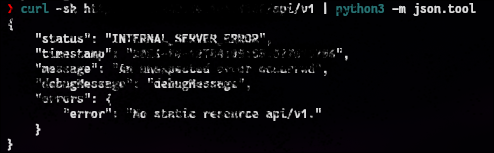
\includegraphics[width=0.82\textwidth]{../evidence/screenshots/100-springboot-internal-server.png}
\captionof*{figure}{\small\textcolor{textmuted}{Respuesta de error con debugMessage en produccion}}
\end{center}

\textbf{Remediacion:}
\begin{itemize}[noitemsep]
  \item Eliminar el campo \texttt{debugMessage} de las respuestas en produccion.
  \item Separar los perfiles de Spring para desarrollo y produccion.
\end{itemize}
\end{tcolorbox}

\vspace{0.4cm}

%% ---- F-C-07 ----
\subsection{F-C-07 --- MySQL 8.0.44 expuesto publicamente}

\begin{tcolorbox}[colback=high!6, colframe=high, boxrule=1pt, arc=3pt,
  title={\textbf{F-C-07} \hfill \textbf{ALTO $\cdot$ CWE-284}},
  fonttitle=\bfseries\color{white}, coltitle=white, colbacktitle=high, breakable]

\textbf{Host:} \texttt{HOST-C:3306}\\[4pt]

\textbf{Descripcion:}
MySQL 8.0.44 es alcanzable directamente desde internet en el puerto 3306.
El acceso como \texttt{root} fue denegado. El riesgo persiste: el puerto
expuesto permite bruteforce de otros usuarios, explotacion de vulnerabilidades
especificas de la version y extraccion de informacion del banner del servicio.

\begin{center}
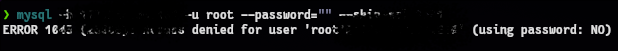
\includegraphics[width=0.82\textwidth]{../evidence/screenshots/100-mysql-root-access-denied.png}
\captionof*{figure}{\small\textcolor{textmuted}{Puerto 3306 accesible --- acceso root denegado}}
\end{center}

\textbf{Remediacion:}
\begin{itemize}[noitemsep]
  \item Restringir el puerto 3306 a conexiones locales o de red interna.
  \item Aplicar regla en el Cloud Firewall del proveedor para bloquear 3306 desde internet.
\end{itemize}
\end{tcolorbox}

\vspace{0.4cm}

%% ---- F-C-08 ----
\subsection{F-C-08 --- SSH root sin proteccion anti-bruteforce}

\begin{tcolorbox}[colback=high!6, colframe=high, boxrule=1pt, arc=3pt,
  title={\textbf{F-C-08} \hfill \textbf{ALTO $\cdot$ CWE-307 / CWE-309}},
  fonttitle=\bfseries\color{white}, coltitle=white, colbacktitle=high, breakable]

\textbf{Host:} \texttt{HOST-C:22}\\[4pt]

\textbf{Descripcion:}
El servicio SSH acepta autenticacion por contrasena para el usuario \texttt{root}.
Durante la prueba se ejecutaron mas de 2000 intentos de autenticacion consecutivos
con hydra sin que el servidor bloqueara la IP ni limitara la tasa de intentos,
confirmando la ausencia de fail2ban o mecanismo equivalente.

\begin{lstlisting}
ssh -v root@HOST-C 2>&1 | grep -i "auth\|method"
hydra -l root -P /usr/share/wordlists/rockyou.txt ssh://HOST-C -t 4 -w 10
# [STATUS] 2000 tries, no lockout triggered
\end{lstlisting}

\begin{center}
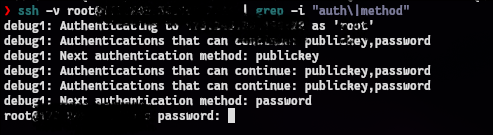
\includegraphics[width=0.82\textwidth]{../evidence/screenshots/100-ssh-root-password-auth-enabled.png}
\captionof*{figure}{\small\textcolor{textmuted}{Autenticacion por contrasena habilitada para root}}
\end{center}

\begin{center}
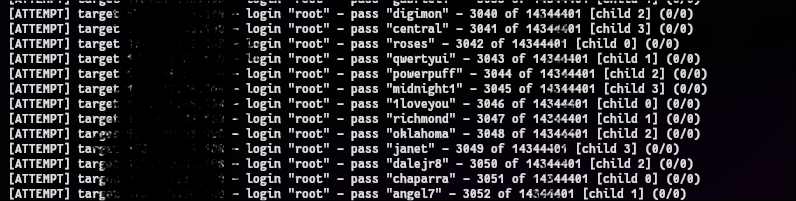
\includegraphics[width=0.82\textwidth]{../evidence/screenshots/100-ssh-bruteforce-hydra-no-lockout.png}
\captionof*{figure}{\small\textcolor{textmuted}{2000+ intentos sin bloqueo de IP ni rate limiting}}
\end{center}

\textbf{Impacto:}
Un atacante puede lanzar un ataque de diccionario indefinidamente contra
\texttt{root}. Con la IP y el usuario obtenidos directamente de la wiki
(F-C-02), el unico factor que previene el compromiso total es la
fortaleza de la contrasena de root.

\textbf{Remediacion:}
\begin{itemize}[noitemsep]
  \item Deshabilitar autenticacion por contrasena: \texttt{PasswordAuthentication no}.
  \item Deshabilitar login root: \texttt{PermitRootLogin no}.
  \item Instalar fail2ban con \texttt{maxretry = 5}, \texttt{bantime = 3600}.
  \item Usar exclusivamente autenticacion por clave publica para SSH.
\end{itemize}
\end{tcolorbox}

\vspace{0.4cm}

%% ---- F-C-09 ----
\subsection{F-C-09 --- UFW deshabilitado --- defensa en profundidad ausente}

\begin{tcolorbox}[colback=medium!10, colframe=medium, boxrule=1pt, arc=3pt,
  title={\textbf{F-C-09} \hfill \textbf{MEDIO $\cdot$ CWE-284}},
  fonttitle=\bfseries\color{white}, coltitle=white, colbacktitle=medium, breakable]

\textbf{Host:} \texttt{HOST-C}\\[4pt]

\textbf{Descripcion:}
Segun la documentacion de infraestructura expuesta en la wiki, UFW esta
inactivo en el servidor de produccion. La politica de iptables INPUT es
\texttt{ACCEPT}. La unica capa de control de acceso de red es el Cloud
Firewall del proveedor. La wiki tambien documenta que Docker bypasea UFW y
que la cadena \texttt{DOCKER-USER} es el unico control para trafico
de contenedores.

\begin{center}
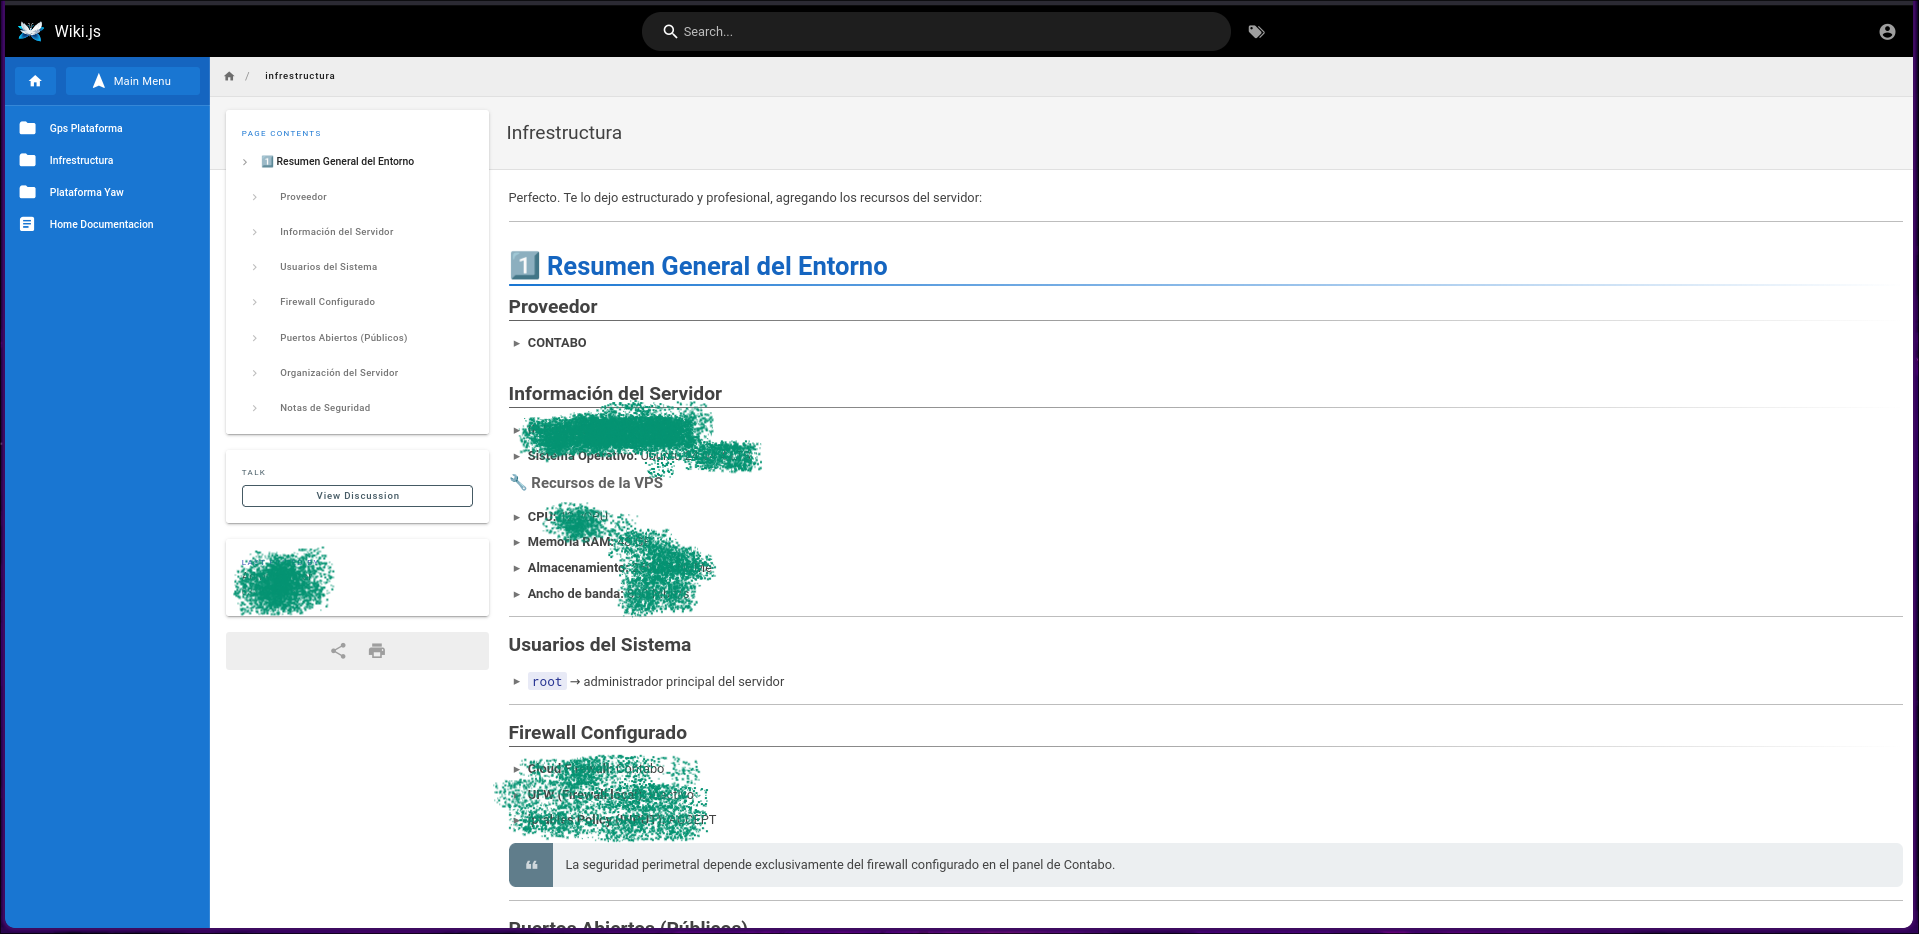
\includegraphics[width=0.82\textwidth]{../evidence/screenshots/100-wikijs-infraestructura-ufw-inactivo.png}
\captionof*{figure}{\small\textcolor{textmuted}{Documentacion interna confirmando UFW inactivo y politica ACCEPT}}
\end{center}

\textbf{Impacto:}
Si el Cloud Firewall del proveedor falla o es mal configurado, todos los puertos
quedan expuestos sin ninguna capa adicional de defensa. El principio de defensa
en profundidad no esta implementado.

\textbf{Remediacion:}
\begin{itemize}[noitemsep]
  \item Activar UFW para servicios del host (SSH, HTTP, HTTPS).
  \item Configurar reglas \texttt{DOCKER-USER} para restringir acceso a puertos de contenedores.
  \item Mantener al menos dos capas de firewall independientes.
\end{itemize}
\end{tcolorbox}

\vspace{0.4cm}

%% ---- F-C-10 ----
\subsection{F-C-10 --- Puertos internos expuestos sin restriccion de IP}

\begin{tcolorbox}[colback=low!6, colframe=low, boxrule=1pt, arc=3pt,
  title={\textbf{F-C-10} \hfill \textbf{BAJO $\cdot$ CWE-284}},
  fonttitle=\bfseries\color{white}, coltitle=white, colbacktitle=low, breakable]

\textbf{Host:} \texttt{HOST-C}\\[4pt]

\textbf{Descripcion:}
Multiples puertos de servicios internos son accesibles directamente desde
internet sin restriccion de IP:

\begin{center}
\begin{tabular}{ll}
\toprule
\textbf{Puerto} & \textbf{Servicio} \\
\midrule
4300            & Spring Boot TCP Server (Actuator abierto) \\
4305            & Spring Boot WebSocket Server (Actuator abierto) \\
4310, 4315      & RTSP (Basic Auth) \\
4350--4360      & Apache Tomcat (401 Unauthorized) \\
5010            & GPS Platform TCP Wialon (Produccion) \\
5020            & GPS Platform TCP Wialon (Desarrollo) \\
5040            & Mall TCP (Produccion) \\
5080            & nginx Mall Trujillo \\
8080            & Wiki.js \\
\bottomrule
\end{tabular}
\end{center}

\begin{center}
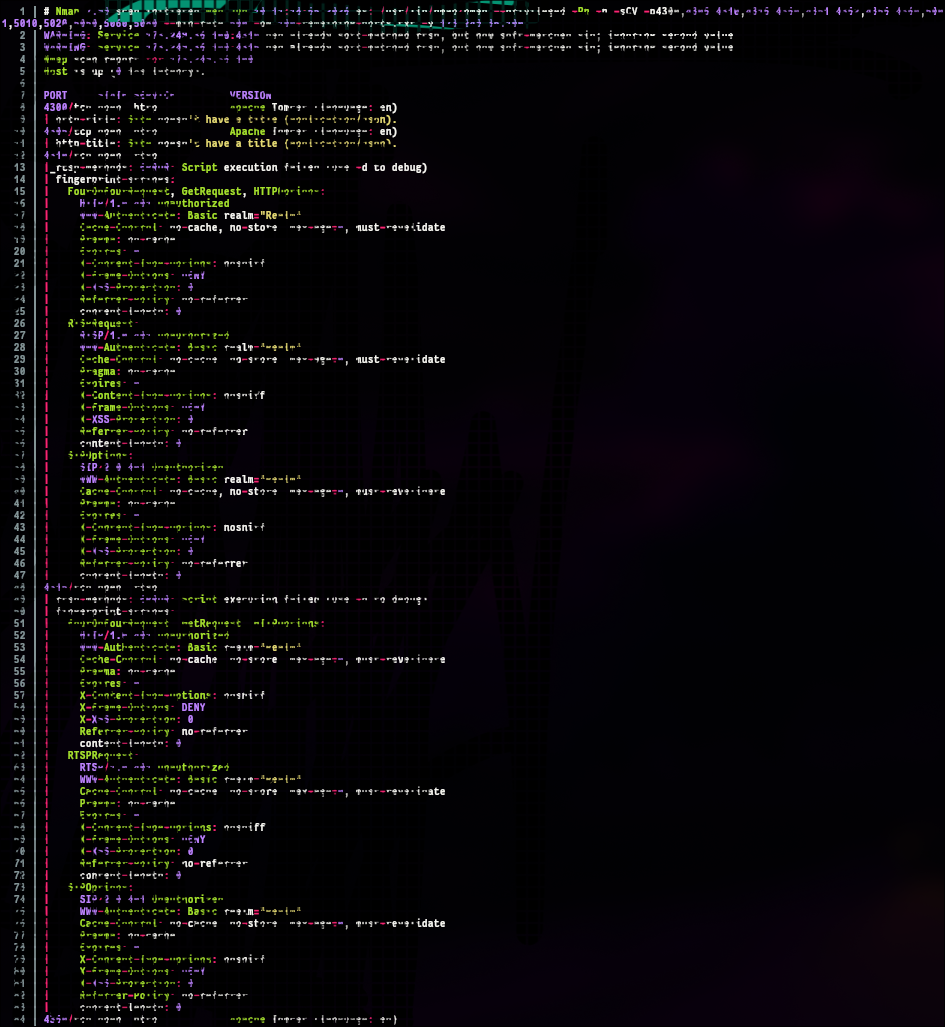
\includegraphics[width=0.82\textwidth]{../evidence/screenshots/100-allservices.png}
\captionof*{figure}{\small\textcolor{textmuted}{Escaneo nmap --- puertos internos accesibles desde internet}}
\end{center}

\textbf{Remediacion:}
\begin{itemize}[noitemsep]
  \item Restringir los puertos internos (4300, 4305, 4350--4360) a IPs autorizadas.
  \item El puerto de desarrollo (5020) no debe ser accesible desde internet.
  \item Aplicar las restricciones via Cloud Firewall del proveedor y reglas \texttt{DOCKER-USER}.
\end{itemize}
\end{tcolorbox}

\vspace{0.4cm}

%% ---- F-C-11 ----
\subsection{F-C-11 --- Certificado SSL expone dominio interno}

\begin{tcolorbox}[colback=lightgray, colframe=bordercolor, boxrule=0.5pt, arc=3pt,
  title={\textbf{F-C-11} \hfill \textbf{INFO $\cdot$ CWE-200}},
  fonttitle=\bfseries, breakable]

\textbf{Host:} \texttt{HOST-C}\\[4pt]

\textbf{Descripcion:}
El certificado SSL expone el dominio interno \texttt{[REDACTED]}
en el campo CN/SAN, permitiendo identificar la infraestructura interna sin
autenticacion ni interaccion con la aplicacion.

\begin{center}
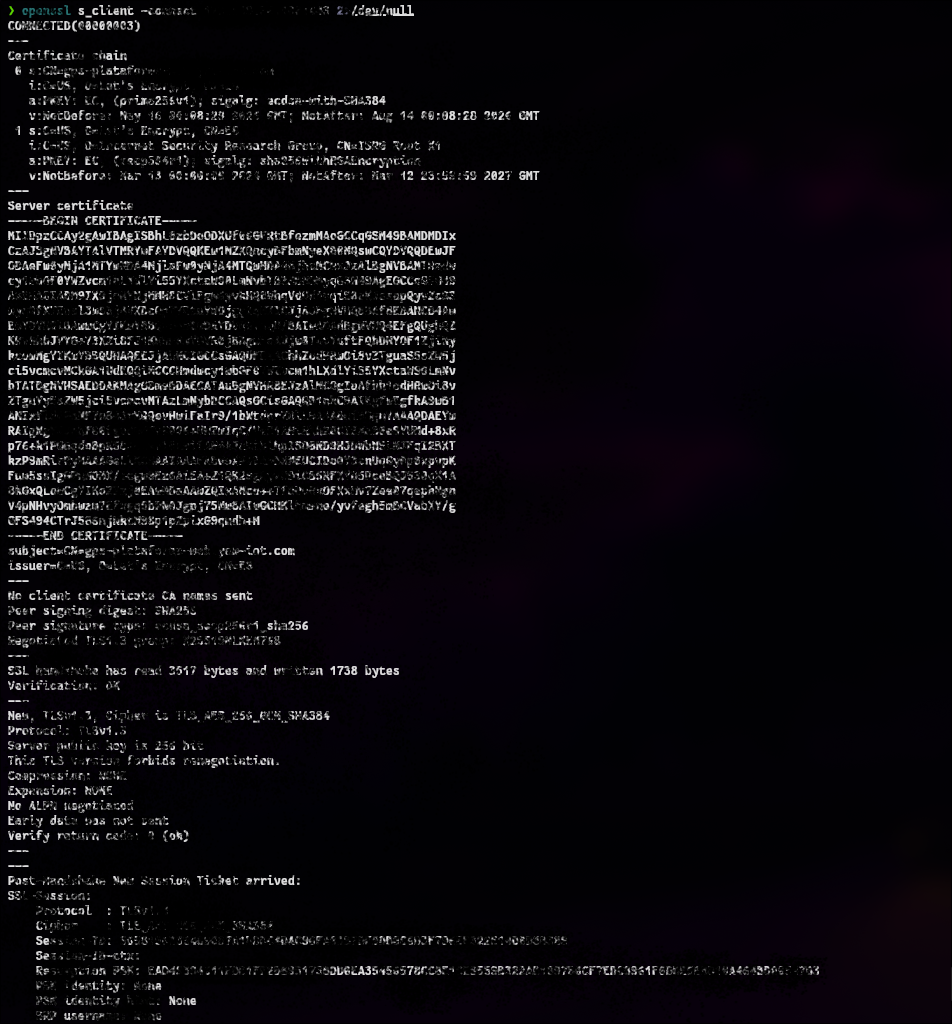
\includegraphics[width=0.82\textwidth]{../evidence/screenshots/100-openssl.png}
\captionof*{figure}{\small\textcolor{textmuted}{Certificado SSL con dominio interno expuesto en CN/SAN}}
\end{center}

\textbf{Remediacion:}
\begin{itemize}[noitemsep]
  \item Separar los certificados internos de los externos.
  \item Usar nombres de dominio genericos para servicios expuestos publicamente.
\end{itemize}
\end{tcolorbox}

\newpage

%% ============================================================
\section{Tabla Consolidada de Hallazgos}
%% ============================================================

\begin{center}
\begin{tabularx}{\textwidth}{llXcc}
\toprule
\textbf{ID} & \textbf{Host} & \textbf{Hallazgo} & \textbf{CVSS} & \textbf{Severidad} \\
\midrule
F-A-01 & A & Version Jenkins expuesta                          & ---  & \cellcolor{lightgray}\textbf{Info} \\
F-A-02 & A & Jenkins CLI accesible sin auth                    & 3.7  & \cellcolor{low!40}\textbf{Bajo} \\
F-A-03 & A & CVE-2024-23897 bloqueado                          & 3.7  & \cellcolor{low!40}\textbf{Bajo} \\
F-B-01 & B & Grafana credenciales por defecto admin:admin      & 9.8  & \cellcolor{critical!80}\textcolor{white}{\textbf{Critico}} \\
F-B-02 & B & Datasources PostgreSQL expuestos en Grafana       & 7.5  & \cellcolor{high!70}\textcolor{white}{\textbf{Alto}} \\
F-B-03 & B & Laravel Debug Mode activo en produccion           & 7.5  & \cellcolor{high!70}\textcolor{white}{\textbf{Alto}} \\
F-B-04 & B & phpMyAdmin Directory Listing habilitado           & 5.3  & \cellcolor{medium!60}\textbf{Medio} \\
F-B-05 & B & MySQL expuesto publicamente en 3306               & 7.5  & \cellcolor{high!70}\textcolor{white}{\textbf{Alto}} \\
F-C-01 & C & Wiki.js publica --- arquitectura interna expuesta & 9.1  & \cellcolor{critical!80}\textcolor{white}{\textbf{Critico}} \\
F-C-02 & C & tunnels.sh con SSH root expuesto en wiki          & 9.8  & \cellcolor{critical!80}\textcolor{white}{\textbf{Critico}} \\
F-C-03 & C & GraphQL Introspection sin autenticacion           & 5.3  & \cellcolor{medium!60}\textbf{Medio} \\
F-C-04 & C & GraphQL stacktrace con rutas internas             & 3.7  & \cellcolor{low!40}\textbf{Bajo} \\
F-C-05 & C & Spring Boot Actuator sin auth --- Redis expuesto  & 5.8  & \cellcolor{medium!60}\textbf{Medio} \\
F-C-06 & C & Spring Boot debugMessage en produccion            & 5.3  & \cellcolor{medium!60}\textbf{Medio} \\
F-C-07 & C & MySQL 8.0.44 expuesto publicamente                & 7.5  & \cellcolor{high!70}\textcolor{white}{\textbf{Alto}} \\
F-C-08 & C & SSH root sin proteccion anti-bruteforce           & 8.1  & \cellcolor{high!70}\textcolor{white}{\textbf{Alto}} \\
F-C-09 & C & UFW deshabilitado --- sin defensa en profundidad  & 5.3  & \cellcolor{medium!60}\textbf{Medio} \\
F-C-10 & C & Puertos internos expuestos sin restriccion de IP  & 3.7  & \cellcolor{low!40}\textbf{Bajo} \\
F-C-11 & C & Certificado SSL expone dominio interno            & ---  & \cellcolor{lightgray}\textbf{Info} \\
\bottomrule
\end{tabularx}
\end{center}

\newpage

%% ============================================================
\section{Recomendaciones Prioritarias}
%% ============================================================

\subsection*{Inmediato --- dentro de 24 horas}

\begin{center}
\begin{tabularx}{\textwidth}{clXl}
\toprule
\textbf{Pri.} & \textbf{ID} & \textbf{Accion} & \textbf{Plazo} \\
\midrule
1 & F-B-01      & Cambiar credenciales de Grafana (admin:admin)          & Inmediato \\
2 & F-C-01      & Habilitar autenticacion obligatoria en Wiki.js         & Inmediato \\
3 & F-C-02      & Eliminar tunnels.sh de la wiki publica                 & Inmediato \\
4 & F-C-08      & Deshabilitar PasswordAuthentication y PermitRootLogin  & 24h \\
5 & F-C-08      & Instalar y configurar fail2ban                         & 24h \\
\bottomrule
\end{tabularx}
\end{center}

\subsection*{Corto plazo --- dentro de 1 semana}

\begin{center}
\begin{tabularx}{\textwidth}{clXl}
\toprule
\textbf{Pri.} & \textbf{ID} & \textbf{Accion} & \textbf{Plazo} \\
\midrule
6  & F-B-05 / F-C-07 & Bloquear MySQL 3306 a red interna via firewall         & 1 semana \\
7  & F-C-05            & Proteger Actuator con Spring Security                  & 1 semana \\
8  & F-B-03            & Configurar APP\_DEBUG=false en Laravel                 & 1 semana \\
9  & F-C-09            & Activar UFW como segunda capa de firewall              & 1 semana \\
10 & F-C-01            & Auditar y rotar credenciales mencionadas en la wiki    & 1 semana \\
\bottomrule
\end{tabularx}
\end{center}

\subsection*{Mediano plazo --- dentro de 1 mes}

\begin{center}
\begin{tabularx}{\textwidth}{clXl}
\toprule
\textbf{Pri.} & \textbf{ID} & \textbf{Accion} & \textbf{Plazo} \\
\midrule
11 & F-C-03      & Deshabilitar GraphQL introspection en produccion       & 1 mes \\
12 & F-C-04/06   & Sanitizar errores: eliminar stacktraces y debugMessage & 1 mes \\
13 & F-C-10      & Restringir puertos internos por IP via Cloud Firewall  & 1 mes \\
14 & F-C-02      & Crear usuarios de deploy sin privilegios root          & 1 mes \\
15 & F-C-01      & Mover la wiki a VPN o red interna exclusivamente       & 1 mes \\
\bottomrule
\end{tabularx}
\end{center}

\newpage

%% ============================================================
\section{MITRE ATT\&CK Mapping}
%% ============================================================

\begin{center}
\begin{tabularx}{\textwidth}{llXl}
\toprule
\textbf{Tactica} & \textbf{Tecnica} & \textbf{Descripcion} & \textbf{Hallazgo} \\
\midrule
Reconnaissance       & T1595.001 & Escaneo nmap de puertos y servicios            & Todos \\
Reconnaissance       & T1596.005 & Certificado SSL para enumeracion de dominios   & F-C-11 \\
Reconnaissance       & T1213     & Wiki.js publica para mapeo de infraestructura  & F-C-01 \\
Initial Access       & T1078.001 & Credenciales por defecto en Grafana            & F-B-01 \\
Credential Access    & T1110.001 & Bruteforce SSH contra usuario root             & F-C-08 \\
Credential Access    & T1552.001 & Credenciales en texto claro en wiki            & F-C-02 \\
Discovery            & T1046     & Escaneo de servicios y puertos expuestos       & F-C-10 \\
Discovery            & T1083     & Directory listing en phpMyAdmin                & F-B-04 \\
Collection           & T1213     & Extraccion de arquitectura interna via wiki    & F-C-01 \\
Collection           & T1530     & Acceso a datasources DB via Grafana            & F-B-02 \\
Defense Evasion      & T1082     & Stacktraces con informacion de sistema         & F-C-04 \\
\bottomrule
\end{tabularx}
\end{center}

\newpage

%% ============================================================
\section{Conclusiones}
%% ============================================================

La evaluacion revelo una superficie de ataque significativa en los tres hosts
evaluados. El servidor principal (\texttt{HOST-C}) concentra el riesgo
mas alto: la exposicion publica de Wiki.js sin autenticacion proporciona a
cualquier atacante externo un mapa completo de la infraestructura, el metodo
de acceso SSH al servidor y la configuracion de servicios criticos, todo sin
necesidad de explotar ninguna vulnerabilidad tecnica.

El hallazgo F-C-02 (tunnels.sh expuesto) es particularmente grave porque
documenta publicamente el vector de acceso al servidor: usuario \texttt{root},
IP publica y estructura de puertos internos. Combinado con F-C-08 (SSH sin
rate limiting), el unico factor que previene el compromiso total del servidor
GPS es la fortaleza de la contrasena de \texttt{root}, que no fue verificable
durante esta evaluacion.

En el Host B, el acceso administrativo completo a Grafana con credenciales
por defecto es un hallazgo que requiere remediacion inmediata: los datasources
PostgreSQL configurados exponen informacion de bases de datos de produccion
que contienen datos GPS reales de los clientes del sistema.

Se recomienda ejecutar las acciones de remediacion inmediata listadas en la
seccion 7 antes de continuar operaciones normales, en particular la habilitacion
de autenticacion en Wiki.js y el cambio de credenciales de Grafana, dado que
ambos son accesibles publicamente desde internet en este momento.

\vspace{0.8cm}

\begin{tcolorbox}[colback=lightgray, colframe=bordercolor, boxrule=0.5pt, arc=3pt]
Este reporte documenta una prueba de penetracion externa autorizada sobre
la infraestructura de la plataforma Cliente GPS IoT, realizada durante el
periodo del [REDACTED]. Todas las pruebas se realizaron
dentro del alcance definido y con autorizacion previa del cliente.

Las tecnicas documentadas \textbf{no deben aplicarse} sobre infraestructura
sin autorizacion explicita y escrita del propietario. El uso no autorizado
puede constituir un delito.

\vspace{0.3cm}
\textit{Clark Espinal --- [REDACTED]}\\
\url{https://clarkportafolio.vercel.app}
\end{tcolorbox}

\end{document}
